\pdfbookmark{Общая характеристика работы}{characteristic}             % Закладка pdf
\section*{Общая характеристика работы}

\newcommand{\actuality}{\pdfbookmark[1]{Актуальность}{actuality}\underline{\textbf{\actualityTXT}}}
\newcommand{\progress}{\pdfbookmark[1]{Разработанность темы}{progress}\underline{\textbf{\progressTXT}}}
\newcommand{\aim}{\pdfbookmark[1]{Цели}{aim}\underline{{\textbf\aimTXT}}}
\newcommand{\tasks}{\pdfbookmark[1]{Задачи}{tasks}\underline{\textbf{\tasksTXT}}}
\newcommand{\aimtasks}{\pdfbookmark[1]{Цели и задачи}{aimtasks}\aimtasksTXT}
\newcommand{\novelty}{\pdfbookmark[1]{Научная новизна}{novelty}\underline{\textbf{\noveltyTXT}}}
\newcommand{\influence}{\pdfbookmark[1]{Практическая значимость}{influence}\underline{\textbf{\influenceTXT}}}
\newcommand{\methods}{\pdfbookmark[1]{Методология и методы исследования}{methods}\underline{\textbf{\methodsTXT}}}
\newcommand{\defpositions}{\pdfbookmark[1]{Положения, выносимые на защиту}{defpositions}\underline{\textbf{\defpositionsTXT}}}
\newcommand{\reliability}{\pdfbookmark[1]{Достоверность}{reliability}\underline{\textbf{\reliabilityTXT}}}
\newcommand{\probation}{\pdfbookmark[1]{Апробация}{probation}\underline{\textbf{\probationTXT}}}
\newcommand{\volumeAndStructure}{\pdfbookmark[1]{Объем и структура работы}{VolumeAndStructure}\underline{\textbf{\volumeAndStructureTXT}}}
\newcommand{\contribution}{\pdfbookmark[1]{Личный вклад}{contribution}\underline{\textbf{\contributionTXT}}}
\newcommand{\publications}{\pdfbookmark[1]{Публикации}{publications}\underline{\textbf{\publicationsTXT}}}
\newcommand{\gratitude}{\pdfbookmark[1]{Благодарности}{gratitude}\section*{\gratitudeTXT}}

{\actuality} 
В последние годы был достигнут значительный прогресс в понимании гипотезы Биркгофа об интегрируемых плоских бильярдах, например, см.~\cite{bm2022}.
С другой стороны, были найдены строгие доказательства неинтегрируемости некоторых бильярдов, таких как эллиптические бильярды в сильном магнитном поле~\cite{bm2020, bm2019}. Неинтегрируемые бильярды, как и бильярды в магнитном поле, исследуются давно, см.~\cite{berry1985, berry1986}.
Изменение бильярдной области с эллипса на, например, стадион, немедленно приводит к хаотической динамике, \cite{bunimovich1974, stockmann2000}.

Хорошо известно, что классический бильярд в ограниченной софокусными квадриками области интегрируем. Интегрируемость  этой системы следует из того, что помимо сохранения полной энергии существует другая постоянная величина, а именно произведение угловых моментов относительно общих фокусов граничных квадрик.
В случае, если фокусы совпадают, степень этого дополнительного интеграла можно понизить, поскольку угловой момент относительно центра круговой области сохраняется.
Однако, в работе \cite{wref13} было показано, что для бильярда в круговом секторе сохраняемой величиной является не  угловой момент, а квадрат углового момента относительно вершины угла.


Недавние работы А.\,Т.~Фоменко и В.\,В.~Ведюшкиной (см. \cite{wref6,wref7,wref8} , а также другие публикации этих авторов) вновь привлекли к этой теме внимание специалистов. 
В частности, в работе \cite{wref6} изучались особенности бильярда в кольце, ограниченном софокусными эллипсами (`эллиптическое кольцо'). В настоящей работе рассматривается соответствующая квантовая система, а именно изучается спектр оператора Шрёдингера в этой области и в ее накрытиях. 
В работе также рассмотрена область (`эллиптический сектор'), ограниченная эллипсом с большой полуосью $0 <r_0$ и эксцентриситетом $\varepsilon$ и 
одной ветвью софокусной гиперболы  (область $A_\varepsilon$)
или двумя ветвями софокусных гипербол (область $B_\varepsilon$).
Все упомянутые эллипсы и гиперболы имеют общие фокусы в точках $(\pm r_0\varepsilon, 0)$.

Для обоих типов областей получены точные решения стационарного уравнения Шрёдингера, а именно собственные функции и соответствующие уровни энергии.

Области $A_\varepsilon$ и $B_\varepsilon$ связаны с бильярдами в круговых секторах следующим образом: при стремлении $\varepsilon$ к 0, обе области стремятся к круговому сектору с некоторым центральным углом. Аналогично, при стремлении $\varepsilon$ к 0 эллиптическое кольцо стремится к круговому кольцу. 

Таким образом, возникает естественный вопрос об установлении асимптотики уровней энергии при $\varepsilon\to 0$. 

{\aim} настоящей работы является получение этой асимптотики с точностью до второго порядка. Ожидается, что в нулевом порядке уровни энергии будут совпадать с результатами~\cite{wref13} для кругового сектора и~\cite[\S~207, с.~276]{wref11} для накрытия кругового кольца кратности $p=1$.

% из первой статьи про косинусное преломление:
%Интерес к составным бильярдам возникает в связи с активно разрабатываемой  в школе А.~Т.~Фоменко теорией бильярдов со сложной топологией, таких как бильярдные книжки. Современное состояние этой теории см. в обзоре [1].  
%
%Рассмотрим ограниченную эллипсом область, разбитую дугой софокусной квадрики на две области с разными плотностями, но постоянными внутри каждой из областей. Тогда мы можем рассмотреть бильярдную траекторию, которая при пересечении границы раздела двух сред меняет направление по закону Снеллиуса [2]: отношение синусов углов падения и преломления равно обратному отношению плотностей сред. 
%Экспериментальная компьютерная проверка демонстрирует, что такой бильярд неинтегрируем. 
%
%С другой стороны, в физике известны законы преломления другого вида. 
%В задачах теплопроводности направление векторов плотностей теплового потока на границе раздела двух сред определяется отношением тангенсов [3, 4].
%В некоторых задачах оптики встречаются законы, формулируемые в терминах отношения косинусов углов падения и преломления [5, 6].
%
%В настоящей работе мы рассматриваем бильярд в эллипсе, разделенном дугами софокусных квадрик на несколько областей $\Omega_i$ с постоянными в них плотностями $n_i$, при этом закон преломления задан равенством $n_1 \cos{\theta_1} = n_2 \cos{\theta_2}$. Мы покажем, что в полученная система будет интегрируемой (см. пункты 5 и 6) и предъявим дополнительный интеграл. В некоторых случаях значения этого дополнительного интеграла принадлежат не прямой, а окружности, см. пункт 7.
Для~достижения поставленной цели необходимо было решить следующие {\tasks}:
\begin{enumerate}[beginpenalty=10000] % https://tex.stackexchange.com/a/476052/104425
  \item Исследовать, разработать, вычислить и~т.\:д. и~т.\:п.
  \item Исследовать, разработать, вычислить и~т.\:д. и~т.\:п.
  \item Исследовать, разработать, вычислить и~т.\:д. и~т.\:п.
  \item Исследовать, разработать, вычислить и~т.\:д. и~т.\:п.
\end{enumerate}

%В настоящей работе  эта асимптотика получена с точностью до второго порядка. В нулевом порядке уровни энергии совпадают с результатами~\cite{wref13} для кругового сектора и~\cite[\S~207, с.~276]{wref11} для накрытия кругового кольца кратности $p=1$.

{\methods} В работе используются элементы теории Штурма и теории специальных функций, методы теории краевых задач и математического анализа

{\novelty} Для уровней энергии получены явные асимптотические выражения, в частности, формулы ($\ref{eq:funcRing}$) и ($\ref{eq:valRing}$) для $p$-листного накрытия эллиптического кольца, а также формулы ($\ref{eq:fun}$) и ($\ref{eq:val}$) для области $A_\varepsilon$ и формулы  ($\ref{eq:funB}$) и ($\ref{eq:valB}$) для области  $B_\varepsilon$. Для особых случаев для областей $A_\varepsilon$ и $B_\varepsilon$ справедливы формулы (\ref{eq:valS1}) и (\ref{eq:valS2}). 
Приведенные асимптотики для собственных значений в зависимости от расстояния между фокусами справедливы с точностью до второго порядка включительно и подтверждаются численными экспериментами.

Интегрируемость классических бильярдов в областях $A_\varepsilon$ и $B_\varepsilon$ следует из существования сохраняющейся величины в дополнение к полной энергии.
В приложении~\ref{app:A} приведен квантовый аналог этой величины, сохраняющейся для квантовых бильярдов в этих же областях.

\begin{enumerate}[beginpenalty=10000] % https://tex.stackexchange.com/a/476052/104425
  \item Впервые \ldots
  \item Впервые \ldots
  \item Было выполнено оригинальное исследование \ldots
\end{enumerate}

{\defpositions}
\begin{enumerate}[beginpenalty=10000] % https://tex.stackexchange.com/a/476052/104425
  \item Первое положение
  \item Второе положение
  \item Третье положение
  \item Четвертое положение
\end{enumerate}
В папке Documents можно ознакомиться с решением совета из Томского~ГУ
(в~файле \verb+Def_positions.pdf+), где обоснованно даются рекомендации
по~формулировкам защищаемых положений.

{\reliability} полученных результатов обеспечивается \ldots \ Результаты находятся в соответствии с результатами, полученными другими авторами.


{\probation}
Основные результаты работы докладывались~на:
перечисление основных конференций, симпозиумов и~т.\:п.

{\contribution} Автор принимал активное участие \ldots

\ifnumequal{\value{bibliosel}}{0}
{%%% Встроенная реализация с загрузкой файла через движок bibtex8. (При желании, внутри можно использовать обычные ссылки, наподобие `\cite{vakbib1,vakbib2}`).
    {\publications} Основные результаты по теме диссертации изложены
    в~XX~печатных изданиях,
    X из которых изданы в журналах, рекомендованных ВАК,
    X "--- в тезисах докладов.
}%
{%%% Реализация пакетом biblatex через движок biber
    \begin{refsection}[bl-author, bl-registered]
        % Это refsection=1.
        % Процитированные здесь работы:
        %  * подсчитываются, для автоматического составления фразы "Основные результаты ..."
        %  * попадают в авторскую библиографию, при usefootcite==0 и стиле `\insertbiblioauthor` или `\insertbiblioauthorgrouped`
        %  * нумеруются там в зависимости от порядка команд `\printbibliography` в этом разделе.
        %  * при использовании `\insertbiblioauthorgrouped`, порядок команд `\printbibliography` в нём должен быть тем же (см. biblio/biblatex.tex)
        %
        % Невидимый библиографический список для подсчёта количества публикаций:
        \phantom{\printbibliography[heading=nobibheading, section=1, env=countauthorvak,          keyword=biblioauthorvak]%
        \printbibliography[heading=nobibheading, section=1, env=countauthorwos,          keyword=biblioauthorwos]%
        \printbibliography[heading=nobibheading, section=1, env=countauthorscopus,       keyword=biblioauthorscopus]%
        \printbibliography[heading=nobibheading, section=1, env=countauthorconf,         keyword=biblioauthorconf]%
        \printbibliography[heading=nobibheading, section=1, env=countauthorother,        keyword=biblioauthorother]%
        \printbibliography[heading=nobibheading, section=1, env=countregistered,         keyword=biblioregistered]%
        \printbibliography[heading=nobibheading, section=1, env=countauthorpatent,       keyword=biblioauthorpatent]%
        \printbibliography[heading=nobibheading, section=1, env=countauthorprogram,      keyword=biblioauthorprogram]%
        \printbibliography[heading=nobibheading, section=1, env=countauthor,             keyword=biblioauthor]%
        \printbibliography[heading=nobibheading, section=1, env=countauthorvakscopuswos, filter=vakscopuswos]%
        \printbibliography[heading=nobibheading, section=1, env=countauthorscopuswos,    filter=scopuswos]}%
        %
        \nocite{*}%
        %
        {\publications} Основные результаты по теме диссертации изложены в~\arabic{citeauthor}~печатных изданиях,
        \arabic{citeauthorvak} из которых изданы в журналах, рекомендованных ВАК%
        \ifnum \value{citeauthorscopuswos}>0%
            , \arabic{citeauthorscopuswos} "--- в~периодических научных журналах, индексируемых Web of~Science и Scopus%
        \fi%
        \ifnum \value{citeauthorconf}>0%
            , \arabic{citeauthorconf} "--- в~тезисах докладов.
        \else%
            .
        \fi%
        \ifnum \value{citeregistered}=1%
            \ifnum \value{citeauthorpatent}=1%
                Зарегистрирован \arabic{citeauthorpatent} патент.
            \fi%
            \ifnum \value{citeauthorprogram}=1%
                Зарегистрирована \arabic{citeauthorprogram} программа для ЭВМ.
            \fi%
        \fi%
        \ifnum \value{citeregistered}>1%
            Зарегистрированы\ %
            \ifnum \value{citeauthorpatent}>0%
            \formbytotal{citeauthorpatent}{патент}{}{а}{}%
            \ifnum \value{citeauthorprogram}=0 . \else \ и~\fi%
            \fi%
            \ifnum \value{citeauthorprogram}>0%
            \formbytotal{citeauthorprogram}{программ}{а}{ы}{} для ЭВМ.
            \fi%
        \fi%
        % К публикациям, в которых излагаются основные научные результаты диссертации на соискание учёной
        % степени, в рецензируемых изданиях приравниваются патенты на изобретения, патенты (свидетельства) на
        % полезную модель, патенты на промышленный образец, патенты на селекционные достижения, свидетельства
        % на программу для электронных вычислительных машин, базу данных, топологию интегральных микросхем,
        % зарегистрированные в установленном порядке.(в ред. Постановления Правительства РФ от 21.04.2016 N 335)
    \end{refsection}%
    \begin{refsection}[bl-author, bl-registered]
        % Это refsection=2.
        % Процитированные здесь работы:
        %  * попадают в авторскую библиографию, при usefootcite==0 и стиле `\insertbiblioauthorimportant`.
        %  * ни на что не влияют в противном случае
        \nocite{vakbib2}%vak
        \nocite{patbib1}%patent
        \nocite{progbib1}%program
        \nocite{bib1}%other
        \nocite{confbib1}%conf
    \end{refsection}%
        %
        % Всё, что вне этих двух refsection, это refsection=0,
        %  * для диссертации - это нормальные ссылки, попадающие в обычную библиографию
        %  * для автореферата:
        %     * при usefootcite==0, ссылка корректно сработает только для источника из `external.bib`. Для своих работ --- напечатает "[0]" (и даже Warning не вылезет).
        %     * при usefootcite==1, ссылка сработает нормально. В авторской библиографии будут только процитированные в refsection=0 работы.
}

При использовании пакета \verb!biblatex! будут подсчитаны все работы, добавленные
в файл \verb!biblio/author.bib!. Для правильного подсчёта работ в~различных
системах цитирования требуется использовать поля:
\begin{itemize}
        \item \texttt{authorvak} если публикация индексирована ВАК,
        \item \texttt{authorscopus} если публикация индексирована Scopus,
        \item \texttt{authorwos} если публикация индексирована Web of Science,
        \item \texttt{authorconf} для докладов конференций,
        \item \texttt{authorpatent} для патентов,
        \item \texttt{authorprogram} для зарегистрированных программ для ЭВМ,
        \item \texttt{authorother} для других публикаций.
\end{itemize}
Для подсчёта используются счётчики:
\begin{itemize}
        \item \texttt{citeauthorvak} для работ, индексируемых ВАК,
        \item \texttt{citeauthorscopus} для работ, индексируемых Scopus,
        \item \texttt{citeauthorwos} для работ, индексируемых Web of Science,
        \item \texttt{citeauthorvakscopuswos} для работ, индексируемых одной из трёх баз,
        \item \texttt{citeauthorscopuswos} для работ, индексируемых Scopus или Web of~Science,
        \item \texttt{citeauthorconf} для докладов на конференциях,
        \item \texttt{citeauthorother} для остальных работ,
        \item \texttt{citeauthorpatent} для патентов,
        \item \texttt{citeauthorprogram} для зарегистрированных программ для ЭВМ,
        \item \texttt{citeauthor} для суммарного количества работ.
\end{itemize}
% Счётчик \texttt{citeexternal} используется для подсчёта процитированных публикаций;
% \texttt{citeregistered} "--- для подсчёта суммарного количества патентов и программ для ЭВМ.

Для добавления в список публикаций автора работ, которые не были процитированы в
автореферате, требуется их~перечислить с использованием команды \verb!\nocite! в
\verb!Synopsis/content.tex!.
 % Характеристика работы по структуре во введении и в автореферате не отличается (ГОСТ Р 7.0.11, пункты 5.3.1 и 9.2.1), потому её загружаем из одного и того же внешнего файла, предварительно задав форму выделения некоторым параметрам

%Диссертационная работа была выполнена при поддержке грантов \dots
\pdfbookmark{Содержание работы}{description}                          % Закладка pdf
\section*{Содержание работы}
Во \underline{\textbf{введении}} формулируется цель работы, кратко излагаются ее результаты и содержание. 
Условно диссертация может быть разделена на две части. Главы 1--2 посвящены исследованию асимптотики собственных значений для квантовых бильярдов на софокусных столах. Главы 3--5 целиком посвящены развитию новой динамической системы, в основе которой лежит косинусный закон преломления траектории.

% актуальность
%исследований, проводимых в~рамках данной диссертационной работы,
%приводится обзор научной литературы по~изучаемой проблеме,
%формулируется цель, ставятся задачи работы, излагается научная новизна
%и практическая значимость представляемой работы. В~последующих главах
%сначала описывается общий принцип, позволяющий \dots, а~потом идёт
%апробация на частных примерах: \dots  и~\dots.

В \underline{\textbf{первой главе}} приведены сведения, необходимые для исследования асимптотики уровней энергии оператора Шрёдингера на софокусных столах при близком к нулю расстоянии между фокусами.
Рассматривается уравнение свободной квантовой частицы с потенциалом <<бесконечной ямы>>. Такой подход устанавливает соответствие между  решениями стационарного уравнения Шрёдингера и собственными  функциями $\psi$ оператора Лапласа с условием Дирихле на границе области $\Omega \subset \mathbb{R}^2$.

Напомним, что в полярной системе координат $(x,y) = (r \cos \phi, r \sin \phi)$ в предположении $\psi(r, \phi) = R(r) \Phi(\phi)$ уравнение Гельмгольца расщепляется в систему дифференциальных уравнений на функции $R(r)$ и $\Phi(\phi)$. В частности, радиальная составляющая $R(r)$ удовлетворяет дифференциальному уравнению Бесселя. 
Ввиду значительной роли функций Бесселя в дальнейших соображениях, в главе приводится основная теория функций Бесселя.
Связь собственных значений оператора Лапласа и нулей функций Бесселя для задачи в полярной системе координат проиллюстрирована на примере свободной квантовой частицы в круге. 
Также приводится анализ задачи в круговом кольце и секторе, поскольку эти области являются предельными для аналогичных областей в эллиптической системе координат $(x,y)=(c \cosh \rho \cos \phi, c \sinh \rho \sin \phi)$ с фокусами в точках $(\pm c,0)$ при $c \to 0$.
Уравнение Гельмгольца в новой системе координат также расщепляется: если $\psi(\rho, \phi) = R(\rho) \Phi(\phi)$, то функции $\Phi(\phi)$ и $R(\rho)$ удовлетворяют \textit{угловому} и \textit{радиальному уравнению Матьё}, соответственно.
Ключевым свойствам решений этих уравнений, \textit{функциям Матьё}, посвящен отдельный раздел первой главы. 
%Приводятся понятия \textit{характеристической экспоненты} $\nu$ из теории Флоке и \textit{характеристических значений} $a_n(q), b_n(q)$ для целого порядка $\nu=n$ и $\lambda_\nu(q)$ для нецелого $\nu$. 
Приводятся элементы теории Флоке и теории Штурма. 
%Глава продолжается приведением необходимой теории функций Матьё. А именно, решение углового уравнения Матьё рассматривается с точки зрения теории Флоке, что позволяет записать решение в виде $F_\nu(\phi) = e^{i \nu \phi} P(\phi)$, где функция $P$ имеет тот же период $\pi$, что и коэффициенты углового уравнения Матьё.
%Из теории Штурма следует ограничение на разделяющий параметр $\zeta$, поскольку при $q\neq 0$ существует не более чем одно периодическое решение с периодом $\pi$ или $2\pi$. А именно, имеет место следующая классификация функций Матьё целого порядка
%\begin{table} [htbp]%
%    \centering
%    \caption{Периодические функции Матьё целого порядка}%
%    \label{tab:table1}% label всегда желательно идти после caption
%	%    \renewcommand{\arraystretch}{1.5}%% Увеличение расстояния между рядами, для улучшения восприятия.
%    \begin{SingleSpace}
%	\begin{tabular}{||c | c | c | c||} 
%            \toprule     %%% верхняя линейка
%            $\zeta$	&   \begin{tabular}{c}Периодическое решение\\ углового уравнения Матьё\footnotemark[3]\end{tabular} &   Период  & Четность функции \\
%            \midrule 
%		$a_{2n}(q)$                   &   $ce_{2n}(z, q)$               & период $\pi$     & четная \\ \hline
%		$a_{2n+1}(q)$                 &   $ce_{2n+1}(z, q)$             & антипериод\footnotemark[4] $\pi$ & четная \\ \hline
%		$b_{2n+1}(q)$                 &   $se_{2n+1}(z, q)$             & антипериод $\pi$ & нечетная \\ \hline          
%		$b_{2n+2}(q)$                 &   $se_{2n+2}(z, q)$             & период $\pi$     & нечетная \\ 
%		            \bottomrule %%% нижняя линейка
%        \end{tabular}%
%    \end{SingleSpace}
%\end{table}
%\footnotetext[3]{В табл. 1 приведены только собственные функции периода $\pi$ или $2\pi$.}
%\footnotetext[4]{Антипериод $\pi$: $f(x+\pi) = -f(x)$.}
%Похожая классификация существует для функций Матьё нецелого порядка, и она также включена в первую главу работы.

%Для нашей задачи основной интерес представляют разложения угловых функций Матьё в ряды Фурье и связь радиальных функций Матьё с угловыми. Как оказывается, радиальные функции допускают запись в виде бесконечной суммы функций Бесселя, при этом коэффициенты в этой сумме будут связаны с коэффициентами Фурье угловой функции Матьё с теми же параметрами $\zeta$ и $q$. 

%Рассматривается также предел характеристических значений $\lambda_\nu(q)$ и собственных функций при $q \to 0$. Аналогичные соображения приведены для непериодических функций Матьё.
%Для радиальных функций Матьё справедливо, что замена $\phi \mapsto i \phi$ превращает угловые уравнения Матьё к радиальным, однако аналогичный ряд по гиперболическим функциям сходится медленно. Но существует разложение радиальных функций Матьё в бесконечную сумму функций Бесселя, где коэффициенты связаны с коэффициентами Фурье угловой функции с теми же параметрами.
%
В отличие от квантового бильярда в круге, в эллипсе появляется дополнительное условие на решения стационарного уравнения Шрёдингера. 
Пусть $\Omega \in \mathbb{R}^2$ и  $J$ -- это часть соединяющего фокусы $(\pm c,0)$ отрезка. Предположим, что $J$ содержится во внутренности области $\Omega$.
Тогда гладкое решение $\psi(\rho,\phi)$ удовлетворяет следующим условиям:
\begin{align}
& \psi(0,\phi) = \psi(0,-\phi)\notag \\
 &   \qquad\qquad\qquad\qquad     \text{\em (непрерывность сдвига через  $J$)} \label{eq:intro_disp}, \\[10pt]
 &   \frac{\partial}{\partial \rho} \psi( \rho, \phi)|_{\rho \to 0} = - \frac{\partial}{\partial \rho} \psi(\rho, - \phi)|_{\rho \to 0} \notag \\
 &\qquad\qquad\qquad\qquad   \text{\em (непрерывность производной через $J$)}\label{eq:intro_grad}, 
\end{align}

Один из разделов первой главы посвящен задаче об асимптотике уровня энергии свободной квантовой частицы в эллипсе с точки зрения теории специальных функций. Эта задача призвана сформировать базовый инструментарий, который получит дальнейшее развитие и применение при рассмотрении задач из следующей главы. В частности, показано, что при $c\to0$ собственные значения в эллипсе имеют своим пределом значения в круге. Этот же характер асимптотического поведения сохраняется и для иных областей, рассмотренных во второй главе.
В завершение первой главы приводится общий вид собственных функций для <<эллиптического кольца>>, анализ задачи продолжен в первом разделе следующей главы.

Асимптотика собственных значений приводится в начале \underline{\textbf{второй главы}}. 
Доказана следующая теорема:
\begin{theorem}
	Значение $\varkappa^2_{k,m}(\delta), k, m \in \mathbb{N}$, зависит от половины фокусного расстояния $\delta$ с точностью до $o(\delta^2)$ следующим образом:
{\small
\begin{equation}
\varkappa^2_{k,m}(\delta) = \left[
\begin{array}{cc}
\dfrac{\alpha_{\nu, m}^2}{r_0^2} + \delta^2 \dfrac{\alpha_{\nu, m}^3}{8 \nu r_0^4} \left. \frac{
\frac{\nu-2}{\nu-1}
\left(
W_{\nu-2, \nu}(u) + W_{\nu, \nu-2}(u)
\right)- 
\frac{\nu+2}{\nu+1}
\left(
W_{\nu+2, \nu}(u) + W_{\nu, \nu+2}(u)
\right)
}{ \frac{\partial W_{\nu,\nu}(u)}{\partial u} }\right|_{u=\alpha_{\nu, m}},  & -\nu \in \mathbb{N} \setminus \{1, 2\}; \\

\dfrac{\alpha_{2, m}^2}{r_0^2} - \delta^2 \dfrac{\alpha_{2, m}^3}{12  r_0^4} \left. \frac{
	\left(
	W_{4, 2}(u) + W_{2, 4}(u)
	\right)
}{ \frac{\partial W_{2,2}(u)}{\partial u} }\right|_{u=\alpha_{2, m}}, & -\nu=2; \\

\dfrac{\alpha_{1, m}^2}{r_0^2} - \delta^2 \dfrac{3 \alpha_{1, m}^3 }{16 r_0^4}
\left. \frac{
	\left(
	W_{3, 1}(u) + W_{1, 3}(u)
	\right)
}{ \frac{\partial W_{1,1}(u)}{\partial u} }\right|_{u=\alpha_{1, m}}, & -\nu=1; \\


\dfrac{\alpha_{0, m}^2}{r_0^2} - \delta^2 \dfrac{\alpha_{0, m}^3}{4r_0^4} \left. \frac{
 \left( W_{2, 0}(u) + W_{0, 2}(u) \right)
}{ \frac{\partial W_{0,0}(u)}{\partial u} }\right|_{u=\alpha_{0, m}}, & \nu=0;   \\

\dfrac{\alpha_{1, m}^2}{r_0^2} - \delta^2 \dfrac{\alpha_{1, m}^3}{16 r_0^4} \left. \frac{ \left( W_{3, 1}(u) + W_{1, 3}(u) \right)
}{ \frac{\partial W_{1,1}(u)}{\partial u} }\right|_{u=\alpha_{1, m}},    & \nu=1;\\

\dfrac{\alpha_{\nu, m}^2}{r_0^2} + \delta^2 \dfrac{\alpha_{\nu, m}^3}{2 r_0^4} \left. \frac{
\frac{1}{4(\nu-1)} \left( W_{\nu-2, \nu}(u) + W_{\nu, \nu-2}(u) \right) - \frac{1}{4(\nu+1)} \left( W_{\nu+2, \nu}(u) + W_{\nu, \nu+2}(u) \right)
}{ \frac{\partial W_{\nu,\nu}(u)}{\partial u} }\right|_{u=\alpha_{\nu, m}},
&   \left[
\begin{aligned}
\nu &\in \mathbb{N} \setminus \{1\},\\
\nu &\notin \mathbb{Z}.
\end{aligned}
\right.
\end{array}
\right.,
%\tag{6}
\label{eq:valRing}
\end{equation}
}
где $\alpha_{\nu, m}$ --- $m$-й нуль функции $W_{\nu, \nu}(u)$. Последняя определяется как $W_{a, b}(u) = Y_a(u)J_b(\lambda u) - Y_a(\lambda u)J_b(u)$ для $\lambda = \frac{r_1}{r_0}$.
\label{th:sect2_th4}
\end{theorem}
Отметим, что при $\delta \to 0$ область приближается к круговому кольцу, а собственные значения совпадают с теми, что были получены для предельной области. 
Большой раздел второй главы посвящен рассмотрению квантовой свободной частицы в областях двух типов: симметричной $A_\varepsilon$ и несимметричной $B_\varepsilon$ (см. рис. \ref{fig:intro_AB_examples}), где симметрия подразумевается относительно горизонтальной оси $Ox$. 
\begin{figure}[ht]
    \begin{minipage}[b][][b]{0.49\linewidth}\centering
        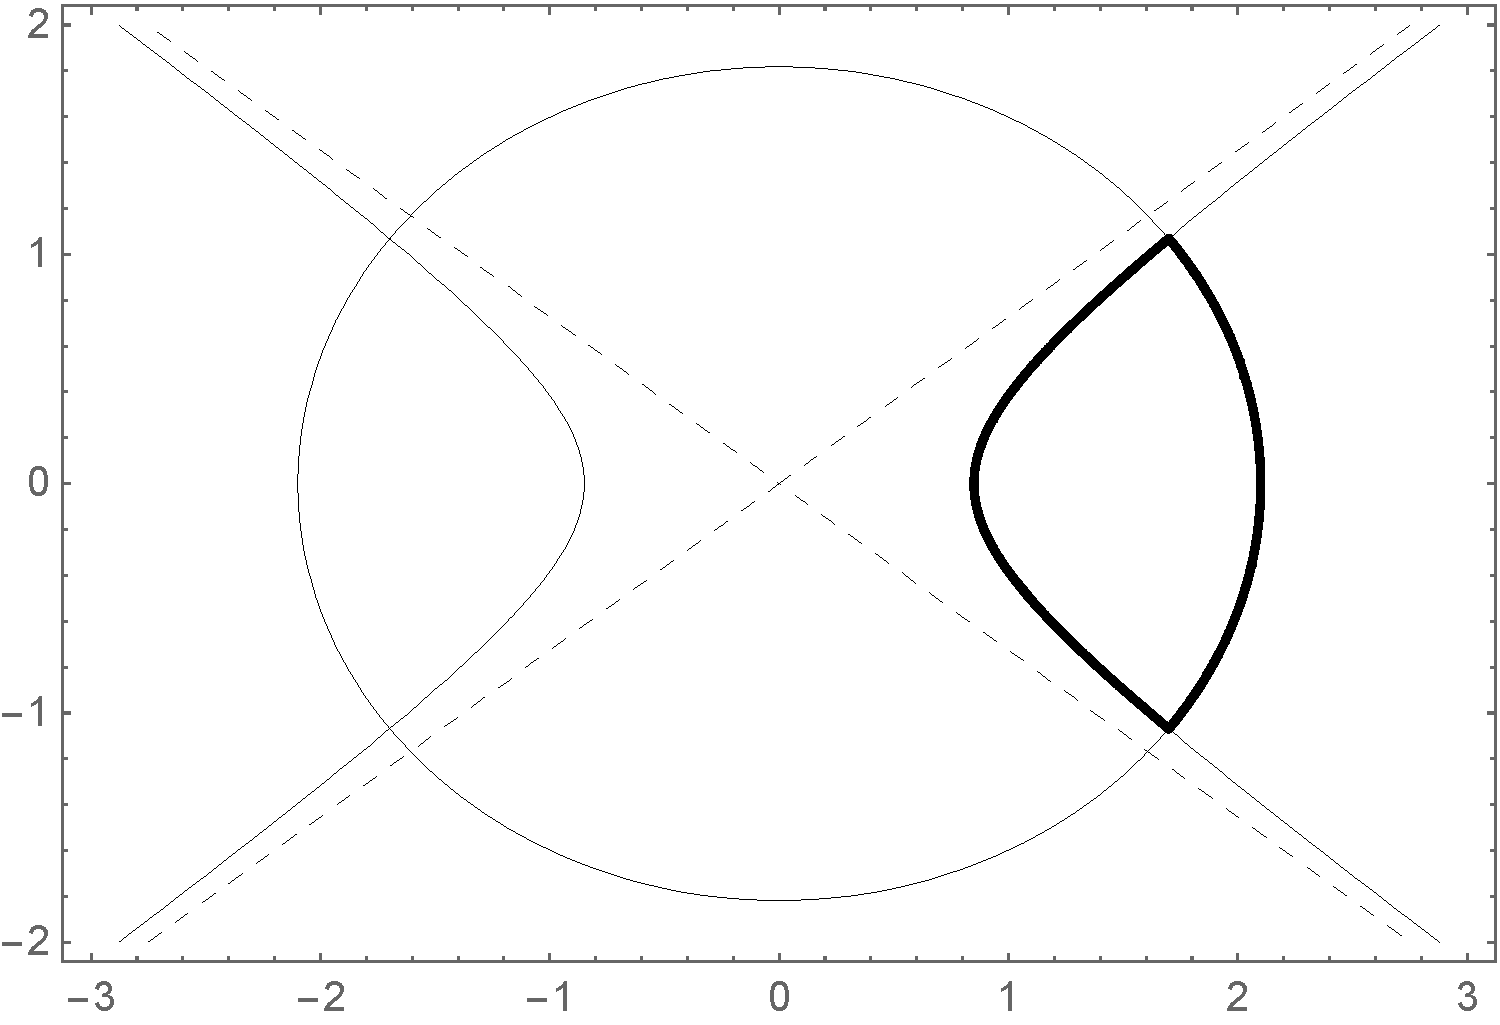
\includegraphics[width=0.8\linewidth]{right1.pdf} \\ 
        Множество $A_\varepsilon$, $\phi_0<\pi/2$
    \end{minipage}
    \hfill
    \begin{minipage}[b][][b]{0.49\linewidth}\centering
        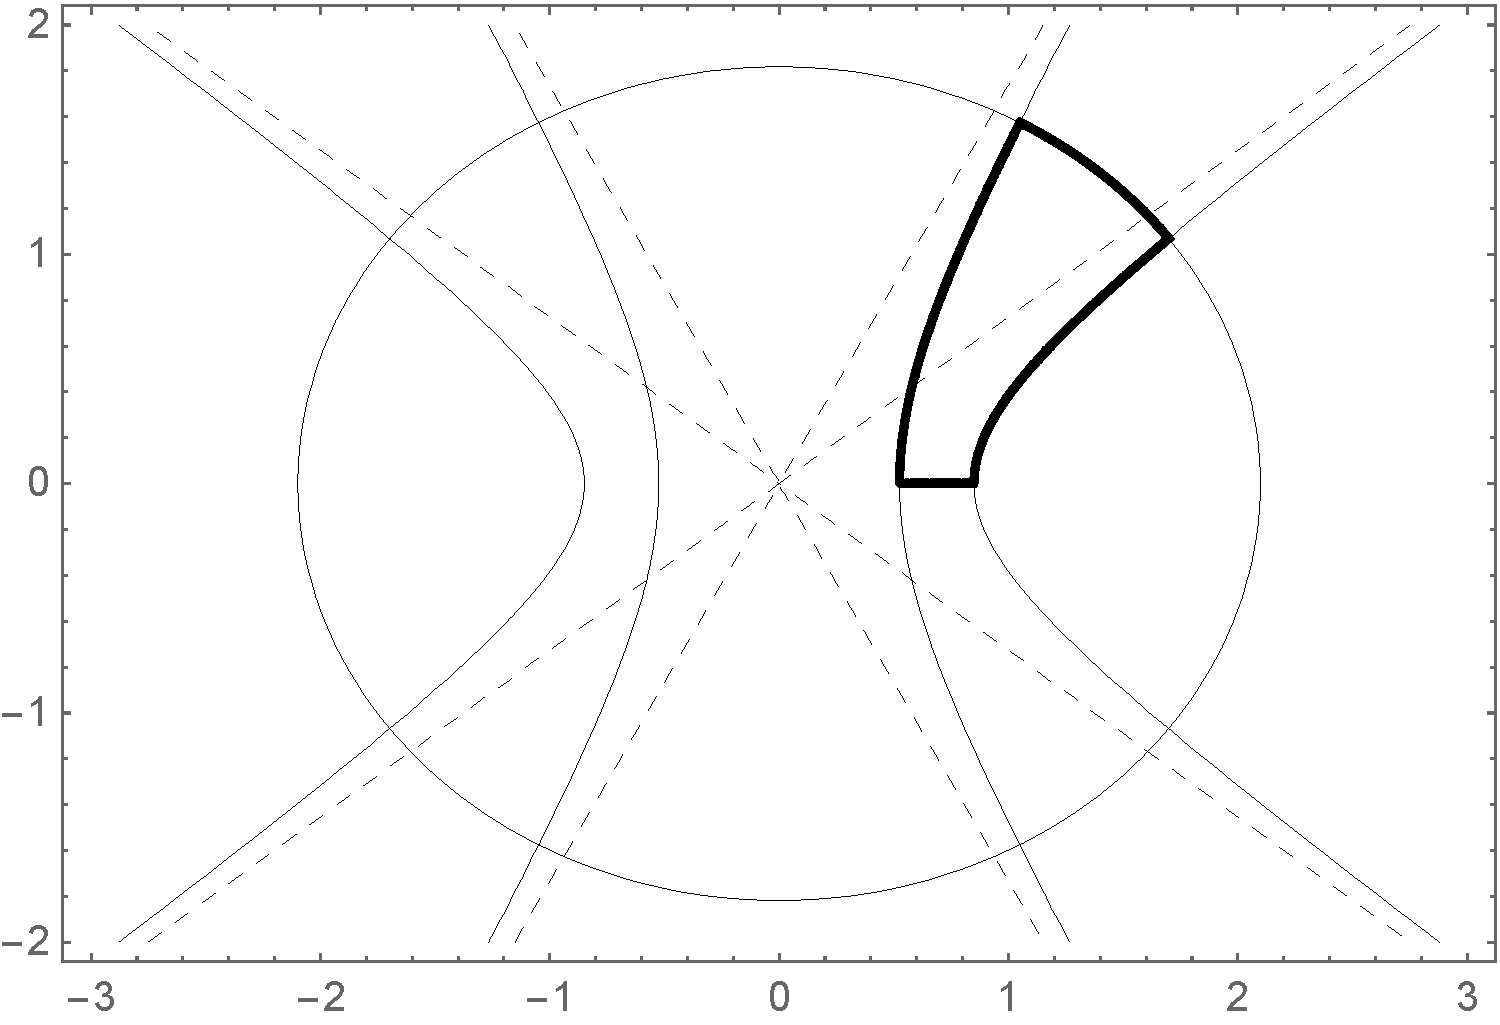
\includegraphics[width=0.8\linewidth]{up1.pdf}  \\
        Множество $B_\varepsilon$, $\phi_0<\phi_1<\pi/2$
    \end{minipage}
\caption{Примеры множеств $A_\varepsilon$ и $B_\varepsilon$.}
\label{fig:intro_AB_examples}
\end{figure}
Обе области при $\delta \to 0$ имеют своим пределом круговой сектор, результат для которого получен в работе \cite{wref13}.

Для симметричной области $A_\varepsilon$ вычислена следующая асимптотика собственных значений:
\begin{theorem} 
Для собственных функций $\psi_{k, m}(\rho, \phi)$ оператора   $\hat{H}$ справедливы выражения
\begin{equation}
\psi_{k, m}(\rho, \phi) = 
\left[
\begin{array}{ll}
    Ce_\nu(\rho, q) ce_\nu(\phi, q) ,   &    \text{нечетный $k \geq 1$}\\
    Se_\nu(\rho, q) se_\nu(\phi, q) ,   &    \text{четный $k \geq 2$}\\
\end{array}
\right.\label{eq:fun}
\end{equation}
с параметрами
\[
\nu = \nu_{k,m} = \nu_0+ \varepsilon^2 \nu_1 + o(\varepsilon^2),  \quad q=q_{k,m} = \dfrac{\varkappa_{k,m}^2 r_0^2 \varepsilon^2}{4},
\]
где
$$\nu_0 = \frac{\pi k}{2\phi_0}\text{\ \  и\  \  }\nu_1=\frac{\alpha_{\nu_0, m}^2}{4} \frac{\pi k \sin 2\phi_0}{\pi^2 k^2 - 4\phi_0^2}  .$$
Для соответствующих собственных  значений  $\varkappa^2_{k, m}$ справедливы равенства
\begin{equation}
\varkappa^2_{k, m} = \dfrac{\alpha_{\nu_0, m}^2}{r_0^2} +
\varepsilon^2 \dfrac{\alpha_{\nu_0, m}^3}{2 r_0^2}\dfrac{\varkappa_1 }{ \left.\frac{\partial J_{\nu_0}(u)}{\partial u}\right|_{u=\alpha_{\nu_0, m}} } + o(\varepsilon^2),\label{eq:val}
\end{equation}
где
\begin{equation*}
    \varkappa_1 = 
    \left[
\begin{array}{ll}
\frac{J_{\nu_0-2}(\alpha_{\nu_0, m})}{4(\nu_0-1)} - \frac{J_{\nu_0+2}(\alpha_{\nu_0, m})}{4(\nu_0+1)} 
  - \nu_1 \left.\frac{\partial J_\nu}{\partial \nu}\right|_{\nu=\nu_0}(\alpha_{\nu_0, m}),\qquad \text{для нечетных $k\geq 3$ ;} \\[10pt]
\frac{(\nu_0 - 2)J_{\nu_0-2}(\alpha_{\nu_0, m})   }{4\nu_0 (\nu_0-1)} -\\
\qquad - \frac{(\nu_0 + 2)J_{\nu_0+2}(\alpha_{\nu_0, m})}{4\nu_0 (\nu_0+1)}  
- \nu_1 \left.\frac{\partial J_\nu}{\partial \nu}\right|_{\nu = \nu_0}(\alpha_{\nu_0, m}), \qquad \ \ \!    \text{для четных $k \geq 2$}.        
\end{array}
\right.
\end{equation*}
Здесь $\alpha_{\nu_0,m}$ --  $m$-й нуль функции Бесселя первого рода $J_{\nu_0}(x)$.
\end{theorem} 
Случай $k=1$ для области $A_\varepsilon$ при $\phi_0=\pi/2$ рассматривается отдельно. Для этого случая формула имеет следующий вид:
\begin{align}
   & \varkappa_{k, m}^2 = \frac{\alpha_{1, m}^2}{r_0^2} - \varepsilon^2 \frac{\alpha_{1, m}^3}{16r_0^2} 
    \frac{J_3(\alpha_{1, m})}{\left.\frac{\partial J_1 (u)}{\partial u}\right|_{u=\alpha_{1, m}}} 
    + o(\varepsilon^2), \label{eq:valS1}
    \end{align}

Для несимметричной области $B_\varepsilon$  аналогичная асимптотика подчиняется следующей формуле:
\begin{theorem}
В области  $B_\varepsilon$ для собственных функций $\psi_{k, m}(\rho, \phi)$ и собственных значений $\varkappa^2_{k, m}$ оператора $\hat{H}$ справедливы выражения

\begin{align}
&\psi_{k, m}(\rho, \phi) = 
    Se_\nu(\rho, q) \biggl( ce_\nu(\phi_0, q) se_\nu(\phi, q) -ce_\nu(\phi, q) se_\nu(\phi_0, q) \biggr) ,  \label{eq:funB}
\end{align}
с параметрами
\begin{align*}    
    & q=q_{k,m} = \frac{\varkappa_{k,m}^2 r_0^2 \varepsilon^2}{4}, \\ 
&\nu = \nu_{k,m} = \frac{\pi k}{\phi_1-\phi_0} +\varepsilon^2 \frac{\alpha_{\nu_0, m}^2}{4} \frac{\pi k (\sin 2\phi_1 - \sin 2 \phi_0)}{\pi^2k^2-(\phi_1-\phi_0)^2} + o(\varepsilon^2) ,  
\end{align*}
где
\begin{align*}
& \nu_0 = \frac{\pi k}{\phi_1-\phi_0},\text{\ \ и \ \ }
\nu_1= \frac{\pi k (\sin 2\phi_1 - \sin 2 \phi_0)}{\pi^2k^2-(\phi_1-\phi_0)^2} .
\end{align*}
Для соответствующих собственных значений справедливы равенства
\begin{align}
\varkappa_{k, m}^2 ={}& \frac{\alpha_{\nu_0, m}^2}{r_0^2} +  \varepsilon^2 \frac{\alpha_{\nu_0, m}^3}{2 r_0^2}\frac{1}{ \left.\frac{\partial J_{\nu_0}(u)}{\partial u}\right|_{u=\alpha_{\nu_0, m}} }  
 \biggl(\frac{(\nu_0 - 2)J_{\nu_0-2}(\alpha_{\nu_0, m})   }{4\nu_0 (\nu_0-1)} -
\notag \\ 
&{}- \frac{(\nu_0 + 2)J_{\nu_0+2}(\alpha_{\nu_0, m})}{4\nu_0 (\nu_0+1)} 
- \nu_1 \left.\frac{\partial J_\nu}{\partial \nu}\right|_{\nu = \nu_0}(\alpha_{\nu_0, m})
    \biggr) + o(\varepsilon^2).\label{eq:valB}
\end{align}
Здесь $\alpha_{\nu_0,m}$ -- $m$-й нуль функции Бесселя первого рода $J_{\nu_0}(x)$.
\end{theorem}

Случай $k=1$ для области $B_\varepsilon$ для $(\phi_0, \phi_1)=(0,\pi)$  рассматривается отдельно. Для нее имеет место следующая формула:
\begin{align}
    \varkappa_{1, m}^2& = \frac{\alpha_{1, m}^2}{r_0^2} - \varepsilon^2 \frac{3\alpha_{1, m}^3}{16r_0^2} 
    \frac{J_3(\alpha_{1, m})}{\left.\frac{\partial J_1 (u)}{\partial u}\right|_{u=\alpha_{1, m}}} 
    + o(\varepsilon^2).  \label{eq:valS2}
\end{align}

В завершение главы приведена постоянная наблюдаемая величина для квантовой свободной частицы на софокусных столах.


\underline{\textbf{Третья глава}} содержит основные понятия теории интегрируемого математического бильярда, а также формулировку косинусного закона преломления.

Приведем косинусный закон преломления как изложено в работе. 
Пусть две области $\Omega_i$ и $\Omega_j$ граничат по кривой $C$. 
Показатели преломления для этих областей равны $n_i$ и $n_j$, соответственно.
Будем считать, что движение материальной точки при достижении кривой $C$ подчиняется следующим правилам (далее мы будем ссылаться на них как на модифицированный закон преломления $(\ast)$).
\begin{itemize}
\item[1.] Выполнено соотношение $n_i \cos \theta_i = n_j \cos \theta_j $, где $\theta_i, \theta_j \in [0,\frac{\pi}{2} ]$ -- углы, которые образуют отрезки траектории   в соответствующих областях с нормалью к кривой $C$, если $\theta_i$ и $\theta_j$ корректно определены.
\item[2.] Если $n_i > n_j$ и материальная точка, двигаясь в области $\Omega_i$, достигает кривой $C$, причем в точке пересечения траектории с кривой $C$ выполнено неравенство $\cos \theta_i > \frac{n_j}{n_i}$, то происходит полное внутреннее отражение траектории в область $\Omega_i$ по закону <<угол падения равен углу отражения>> (в этом случае угол $\theta_j$ не определен, поскольку $\frac{n_i}{n_j} \cos \theta_i > 1$). 
\item[3.] В предыдущих двух пунктах два соседних отрезка траектории с общей точкой на кривой $C$ лежат по разные стороны от нормали к кривой $C$ в этой точке.
\item[4.] Если $n_i > n_j$ и материальная точка, двигаясь в области $\Omega_j$, достигает кривой $C$, причем $\theta_j = 0$, тогда $\cos \theta_i = \frac{n_j}{n_i}$ и материальная точка продолжает движение в области $\Omega_i$ вдоль любого из двух возможных направлений, образующих угол $\theta_i$ с нормалью к кривой $C$.
\item[5.] Аналогично при $n_i < n_j$.
\end{itemize}

\begin{figure}[!htb]
\minipage{0.32\textwidth}
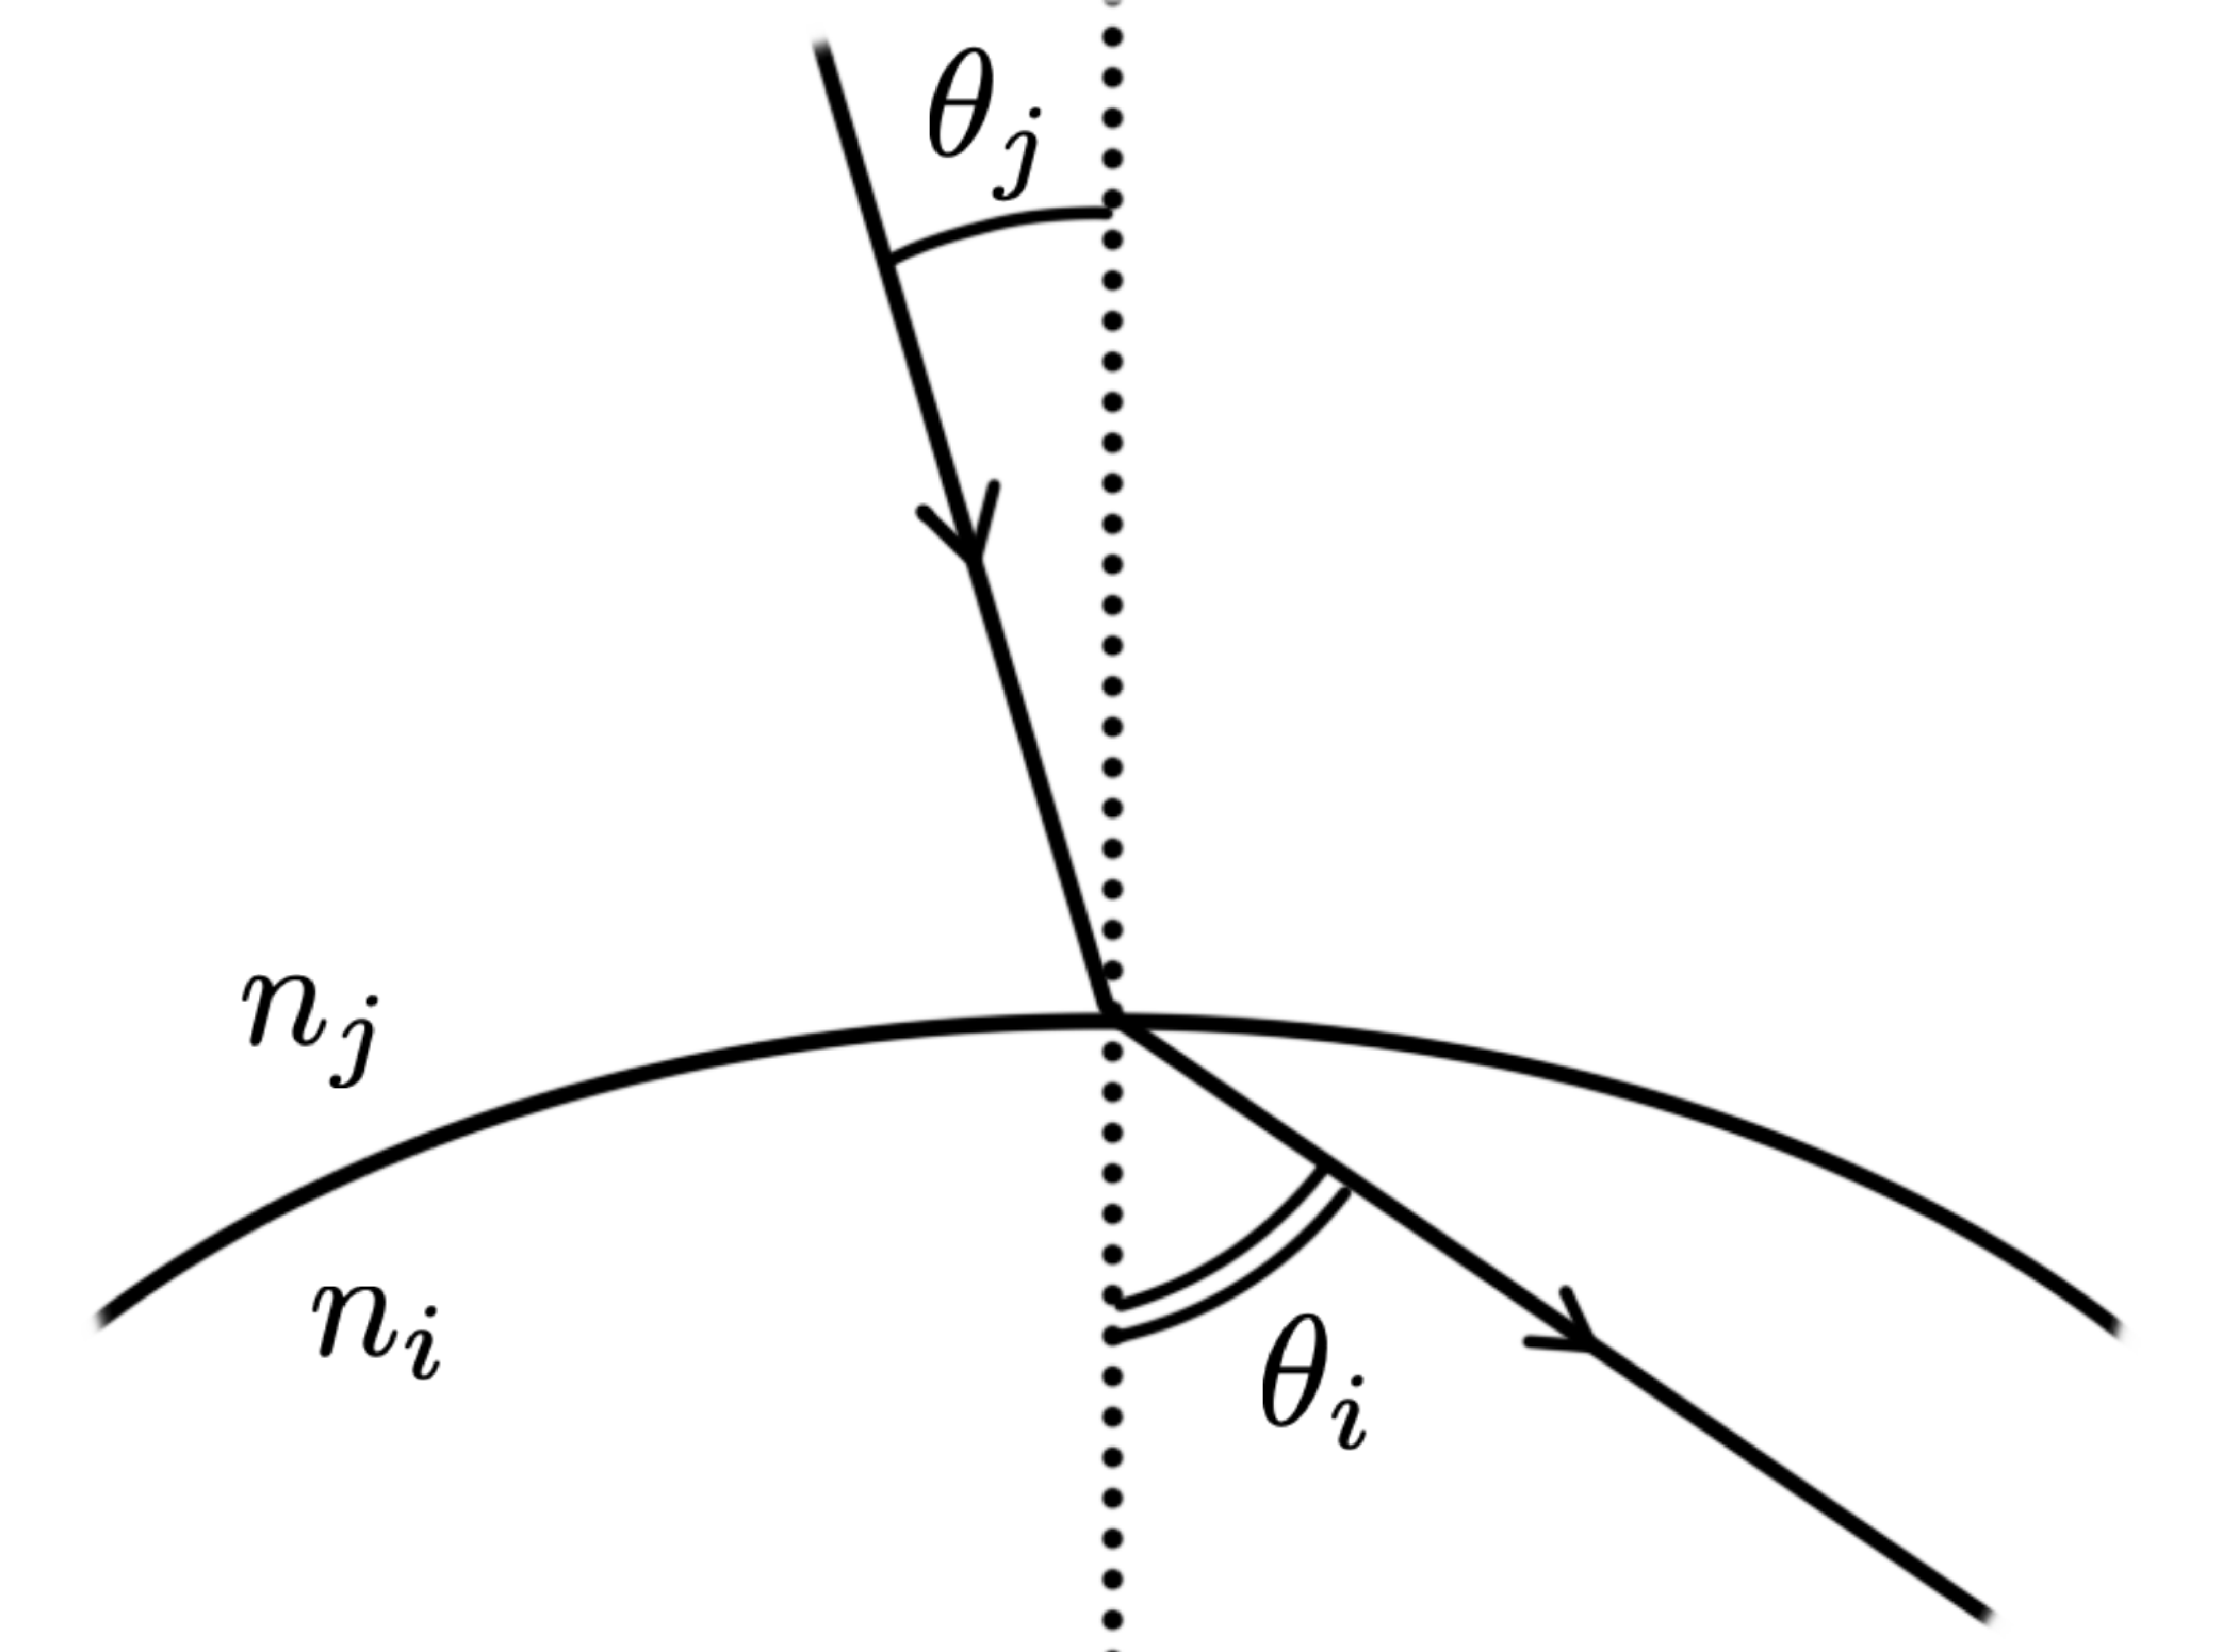
\includegraphics[width=\linewidth]{images/ch4/section1/example1.pdf}
    \caption{Иллюстрация к пункту 1.}
    \label{fig:intro_example1}
\endminipage\hfill
\minipage{0.32\textwidth}
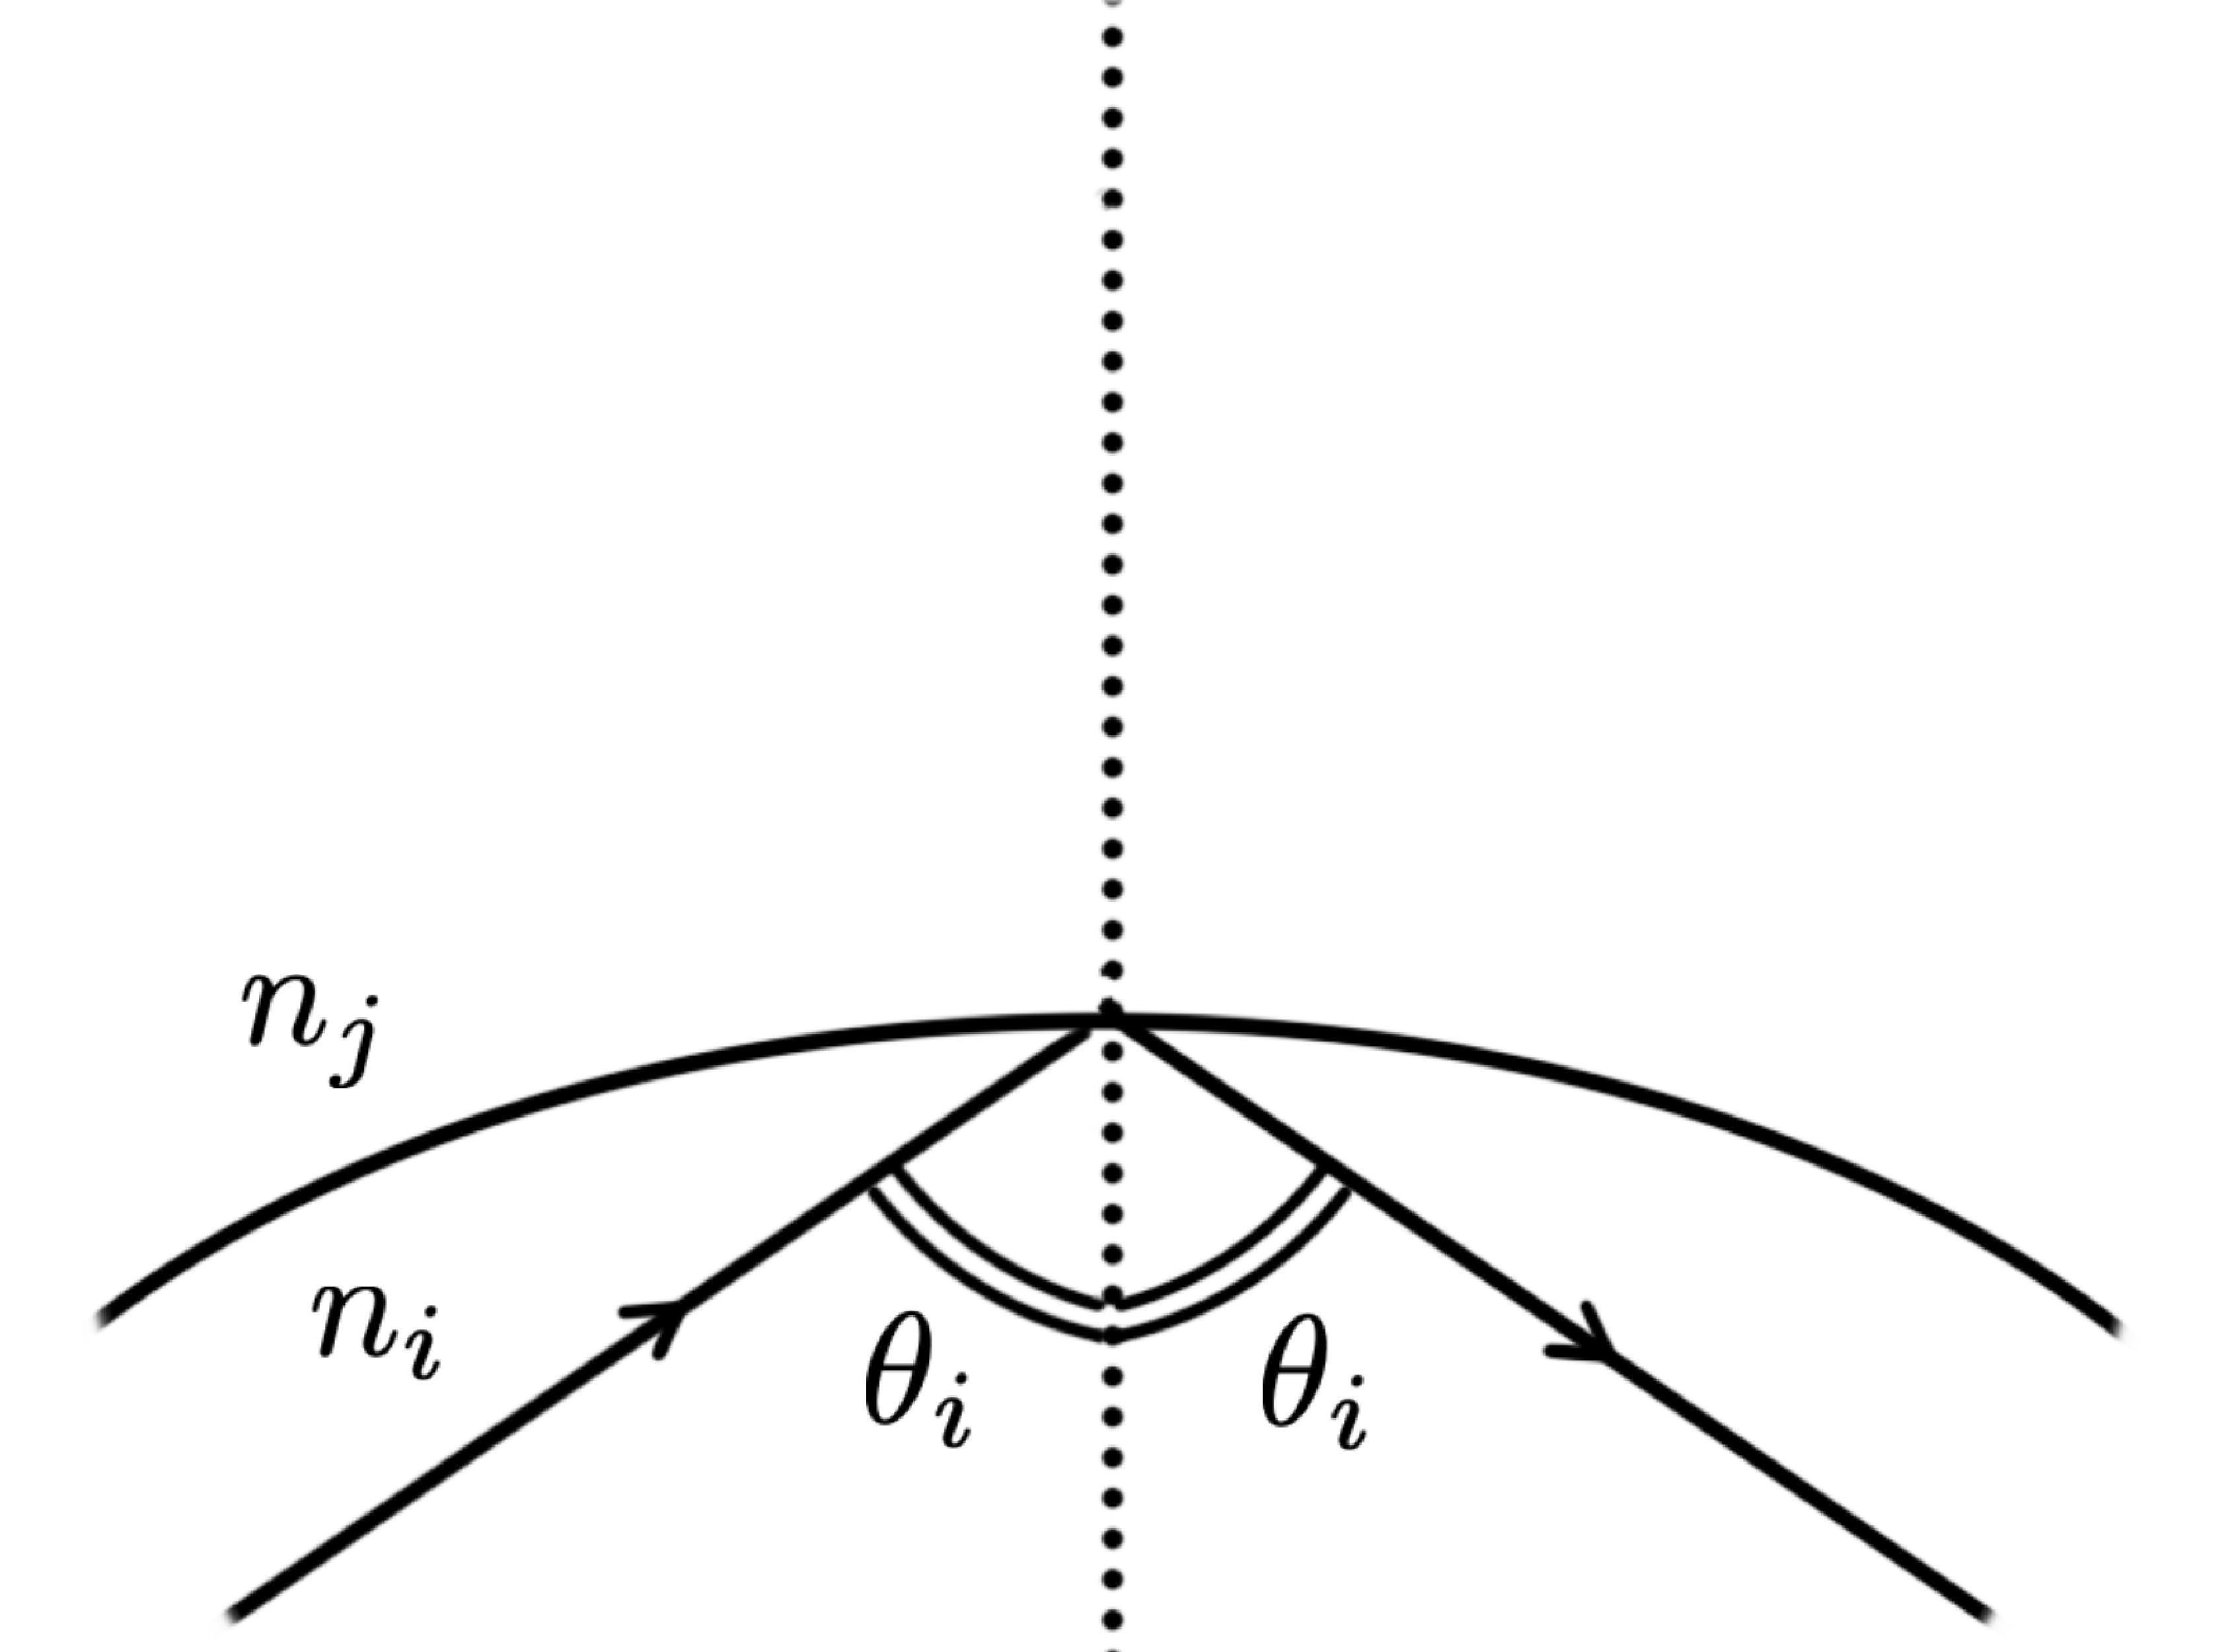
\includegraphics[width=\linewidth]{images/ch4/section1/example2.pdf}
    \caption{Иллюстрация к пункту 2.}
    \label{fig:intro_example2}
\endminipage\hfill
\minipage{0.32\textwidth}
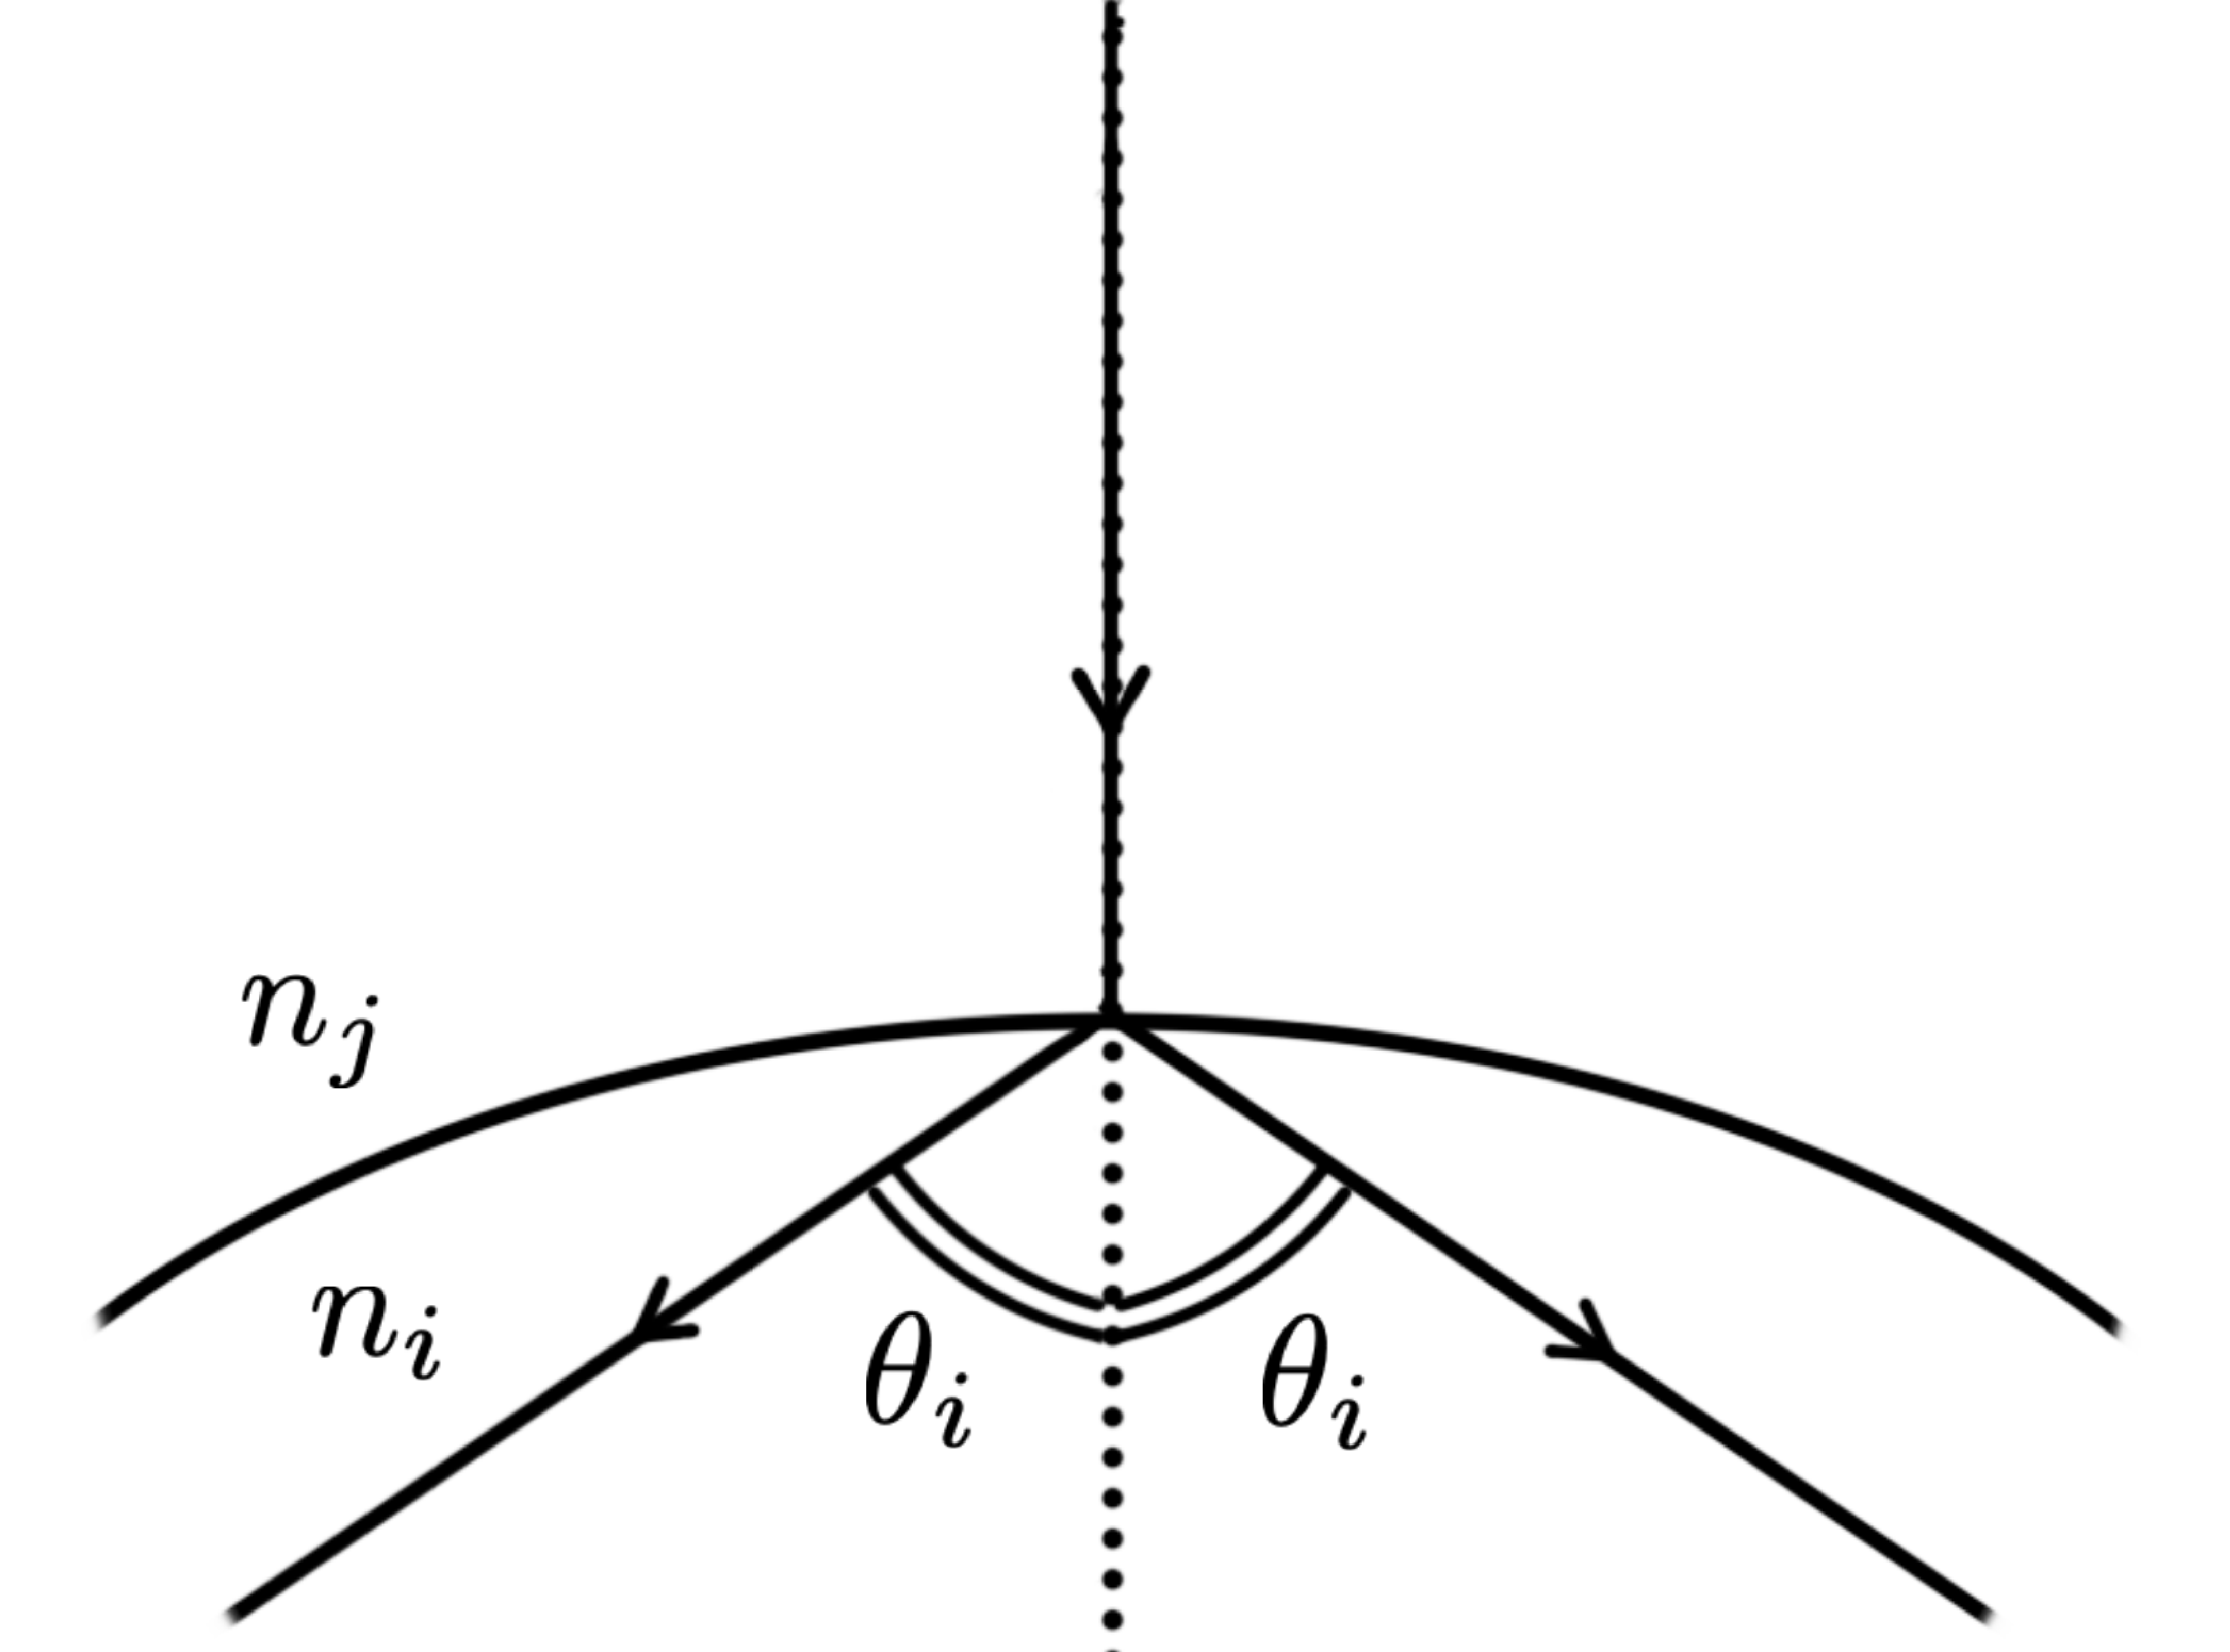
\includegraphics[width=\linewidth]{images/ch4/section1/example3.pdf}
    \caption{Иллюстрация к пункту 4.}
    \label{fig:intro_example3}
\endminipage\hfill
\end{figure}

Под \textit{софокусным столом} будем понимать область, ограниченную дугами эллипсов и гипербол с общими фокусами в точках $(\pm c, 0)$, $c > 0$. В частности каждая из \textit{софокусных квадрик} $Q_\lambda$ удовлетворяет уравнению $\dfrac{x^2}{a^2-\lambda} +\dfrac{y^2}{b^2-\lambda} = 1$ для некоторого параметра  $\lambda \in (0, a^2)$.
В теории классического математического бильярда в эллипсе в качестве постоянной движения часто рассматривают параметр \textit{каустики} -- такой софокусной квадрики, которая является касательной к каждому звену бильярдной траектории. Этот параметр может быть вычислен явно как функция координат точки и компонент вектора скорости:
$$\Lambda(x, y, v_x, v_y) =  \dfrac{a^2 v_y^2 + b^2v_x^2 - (x v_y-y v_x)^2}{v_x^2 + v_y^2}.$$

Для бильярдов на софокусных столах, подчиняющихся этому закону, приводится выражение для постоянной движения.
А именно, если преломление по закону $(\ast)$ происходит на дугах непересекающихся квадрик $Q_1, \ldots, Q_k$, тогда справедливо следующее утверждение:

\begin{theorem}
Пусть внутренность эллипса разбита попарно непересекающимися дугами софокусных квадрик на области $\Omega_1, \ldots, \Omega_k$. Перенумеруем области так, чтобы общие границы имели только области с соседними номерами. Пусть $\lambda_j$ -- параметр софокусной квадрики, разделяющей $\Omega_j$ и $\Omega_{j+1}$, $j=1, \ldots, k-1$. Здесь и далее показатель преломления для области $\Omega_j$ обозначается через $n_j$.
Определим функцию $\Xi(x, y, v_x, v_y)$ по формуле: 
\begin{equation*}
\Xi(x, y, v_x, v_y) = \left[
\begin{array}{ll}
    \Lambda(x, y, v_x, v_y) n_1^2, \qquad  \ \ \qquad   \text{ если } (x,y) \in \Omega_1 ;
    \\
    \Lambda(x, y, v_x, v_y) n_p^2 + \sum_{j=1}^{p-1} \lambda_j(n_j^2-n_{j+1}^2), \\
     \qquad \qquad \qquad \qquad \qquad \qquad  \text{ если } (x,y) \in \Omega_p \text{ для } 1 < p \leq k. 
\end{array}
\right.
\end{equation*}
Функция $\Xi(x, y, v_x, v_y)$ является константой на траекториях бильярда с косинусным законом преломления $(\ast)$.
\label{th:intro_non_intersecting}
\end{theorem}

Два возможных варианта таких разбиений показаны на рис. \ref{fig:intro_example4} и \ref{fig:intro_example5}. 
\begin{figure}[!htb]
\minipage{0.45\textwidth}
   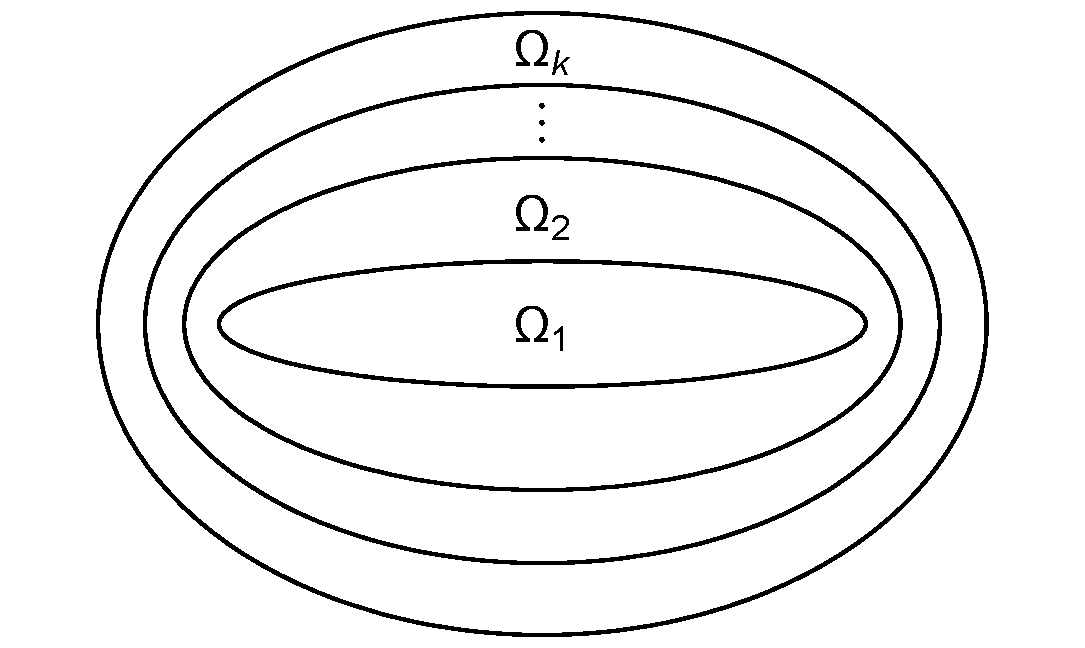
\includegraphics[width=1\textwidth]{images/ch4/section1/multiple ellipses.pdf}
    \caption{Взаимное расположение областей $\Omega_1, \ldots, \Omega_k$.}
    \label{fig:intro_example4}
\endminipage\hfill
\minipage{0.45\textwidth}
    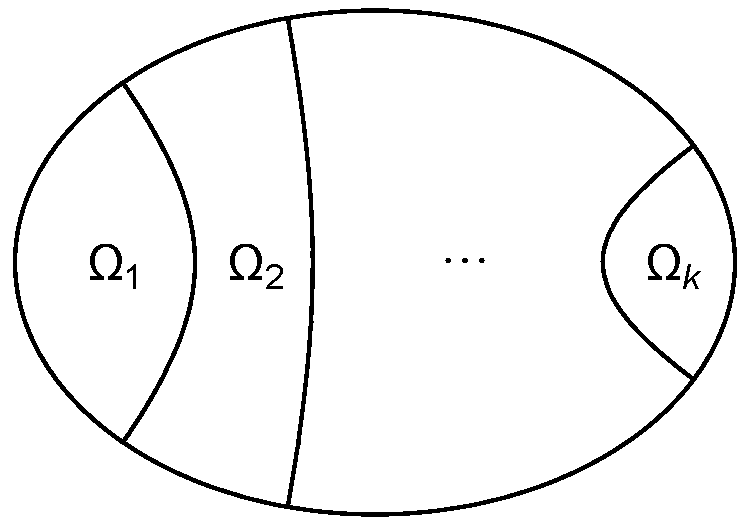
\includegraphics[width=0.9\textwidth]{images/ch4/section1/multiple hyperbolas.pdf}   
    \caption{Взаимное расположение областей $\Omega_1, \ldots, \Omega_k$.}
    \label{fig:intro_example5}
\endminipage\hfill
\end{figure}
Возникает \textbf{задача А}:  описать слоение изоэнергитического многообразия на поверхности уровня первого интеграла $\Xi$ для случаев, показанных на рис. \ref{fig:intro_example4} и \ref{fig:intro_example5}. В следующей главе подробно рассматривается случай двух областей, разделенных одним софокусным эллипсом (см. рис. \ref{fig:intro_example4} при $k=2$). Динамика этой системы и перестройки поверхностей постоянного значения интеграла $\Xi$ уже в этом случае очень нетривиальны.

Случай пересекающихся квадрик оказывается гораздо сложнее. Каждой точке $A$ пересечения разделяющих среды квадрик требуется поставить в соответствие коэффициент $\gamma_A$, имеющий смысл \textit{коэффициента ветвления}. Величина $\gamma_A$ явно зависит от параметров пересекаюшихся в точке $A$ квадрик и параметров $n_j$ примыкающих областей $\Omega_j$.

%В частности, дополнительный интеграл принимает значения не в $\mathbb{R}$, а в фактор-группе $\mathbb{R}$ по  аддитивной подгруппе, допускающей явное описание.
%Если существует единственная точка пересечения преломляющих квадрик, первый интеграл $\Xi$ из теоремы формулируется иначе.
\begin{figure}[!htb]
\centering
     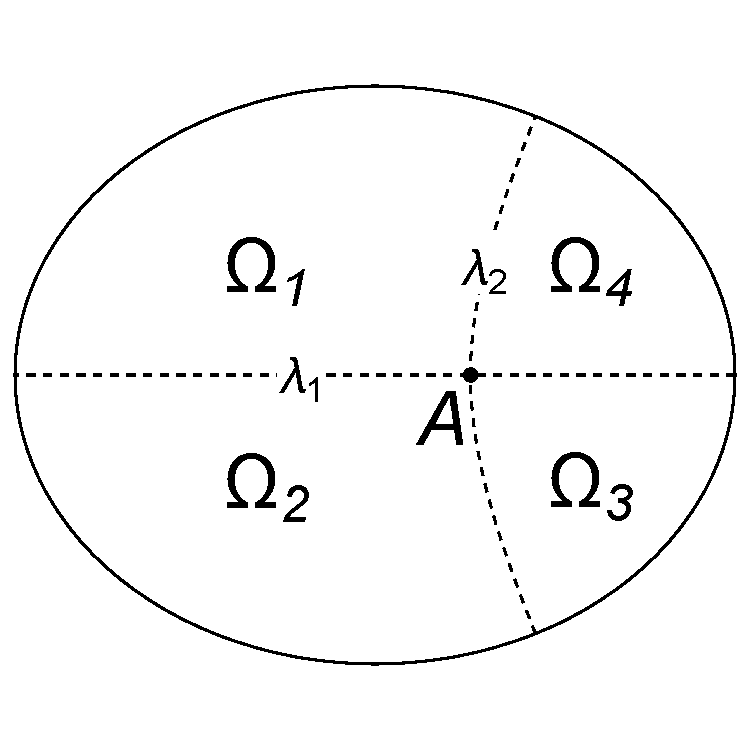
\includegraphics[width=0.35\textwidth]{images/ch4/section1/img2.pdf}
\caption{Взаимное расположение областей $\Omega_1,\ldots,\Omega_4$.}
    \label{fig:intro_example6}
\end{figure}

К примеру, для области с изображенным на рис. \ref{fig:intro_example6} разбиением введем коэффициент $\gamma_A$ в точке $A$, имеющий смысл коэффициента ветвления, по формуле $$\gamma_A = (\lambda_1 - \lambda_2) ( n_1^2 - n_2^2 + n_3^2 - n_4^2).$$

Определим вспомогательную функцию $\widetilde{\Xi}(x, y, v_x, v_y)$ 

\begin{equation*}
\widetilde{\Xi}(x, y, v_x, v_y) = \left[
\begin{array}{ll}
    \Lambda(x, y, v_x, v_y) n_1^2, \qquad  \  \ \qquad   \text{ если } (x,y) \in \Omega_1 
    \\
    \Lambda(x, y, v_x, v_y) n_p^2 + \sum_{j=1}^{p-1} \lambda_{\sigma(j)}(n_j^2-n_{j+1}^2), \\
     \qquad \qquad \qquad \qquad \qquad \qquad  \text{ если } (x,y) \in \Omega_p \text{ для } 1 < p \leq 4,
\end{array}
\right.
\end{equation*}
где $\sigma(j)$ -- номер квадрики, разделяющей $\Omega_j$ и $\Omega_{j+1}$. 
Неформально говоря, величина $\widetilde{\Xi}$ почти подходит на роль дополнительного интеграла, но имеет разрыв на дуге, разделяющей области $\Omega_1$ и $\Omega_4$. Можно проверить, что на любой бильярдной траектории, пересекающей эту дугу, функция $\widetilde{\Xi}$ испытывает один и тот же скачок, равный  $\pm \gamma_A$. 
Поэтому мы определим \textit{первый интеграл $\Xi(x, y, v_x, v_y)$ со значениями в $S^1= \mathbb{R}/\gamma_A \mathbb{Z}$ }по формуле $$\Xi(x, y, v_x, v_y) = \widetilde{\Xi}(x, y, v_x, v_y) \mod \gamma_A.$$
Эта величина на траекториях бильярда сохраняется.
Аналогичный подход справедлив и в других случаях единственной точки пересечения квадрик, на которых происходит преломление по правилу $(\ast)$.

Если границы раздела областей пересекаются по двум и более точкам, то имеет место общая закономерность: 
\textit{ 
\noindent Для каждой точки пересечения $A_i, i=1,\ldots,m$, определен коэффициент $\gamma_{A_i}$. Дополнительный интеграл \  $\Xi(x, y, v_x, v_y)$ принимает значения в $\mathbb{R}/(\gamma_{A_1} \mathbb{Z}+ \ldots + \gamma_{A_m} \mathbb{Z})$. Если $\gamma_{A_i}$ соизмеримы, т. е. всевозможные дроби $\dfrac{\gamma_{A_i}}{\gamma_{A_j}}$ --- рациональные числа (или бесконечность), то $\mathbb{R}/(\gamma_{A_1} \mathbb{Z}+ \ldots + \gamma_{A_m} \mathbb{Z}) = S^1$. Если же среди $\gamma_{A_i}$ есть пара с иррациональным отношением $\dfrac{\gamma_{A_i}}{\gamma_{A_j}}$, то подгруппа $\gamma_{A_1} \mathbb{Z}+ \ldots + \gamma_{A_m} \mathbb{Z}$ всюду плотна в $\mathbb{R}$. В этом случае дополнительный интеграл $\Xi(x, y, v_x, v_y)$ корректно определен, но использовать его для топологического анализа структуры траекторий представляется весьма затруднительным.}

%\begin{figure}[!htb]
%\centering
%   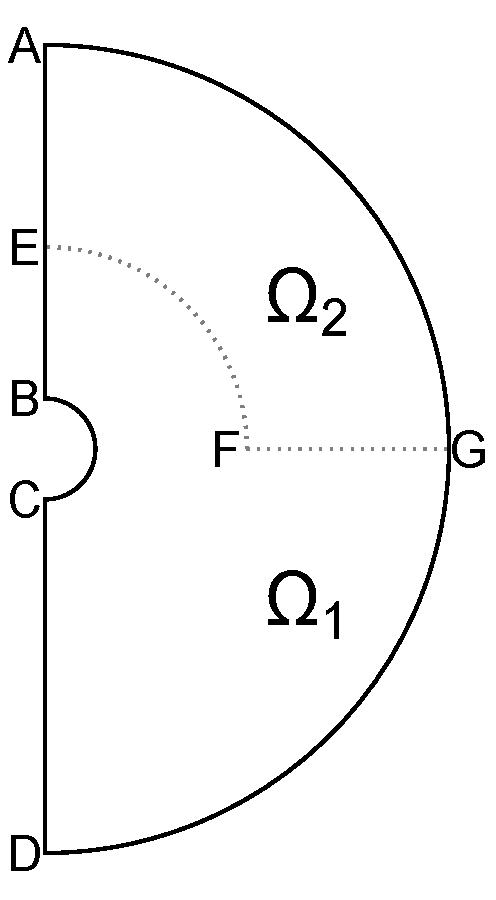
\includegraphics[width=0.2\textwidth]{images/ch4/section1/imgB.pdf}   
%    \caption{Взаимное расположение областей $\Omega_1, \Omega_2$.}
%    \label{fig:intro_example9}
%\end{figure}
%
%В рамках задачи Б будет рассмотрен в качестве бильярдной области $\Omega$  <<прямоугольник>>, изображенный на рис. \ref{fig:intro_example9}. Требуется описать как изоэнергетическое многообразие расслаивается на поверхности уровня первого интеграла $\Xi$.
%
%Можно сослаться на свои работы в автореферате. Для этого в файле
%\verb!Synopsis/setup.tex! необходимо присвоить положительное значение
%счётчику \verb!\setcounter{usefootcite}{1}!. В таком случае ссылки на
%работы других авторов будут подстрочными.
%Изложенные в третьей главе результаты опубликованы в~\cite{vakbib1, vakbib2}.
%Использование подстрочных ссылок внутри таблиц может вызывать проблемы.
%


\underline{\textbf{Четвертая глава}} посвящена рассмотрению задачи А: описать слоение изоэнергетического многообразия на поверхности уровня первого интеграла $\Xi$ для подчиняющейся закону $(\ast)$ бильярдной системы в области $\Omega = \Omega_{in} \cup \Omega_{out}$ (см. рис. \ref{fig:intro_problemA}).
\begin{figure}[!htb]
\centering
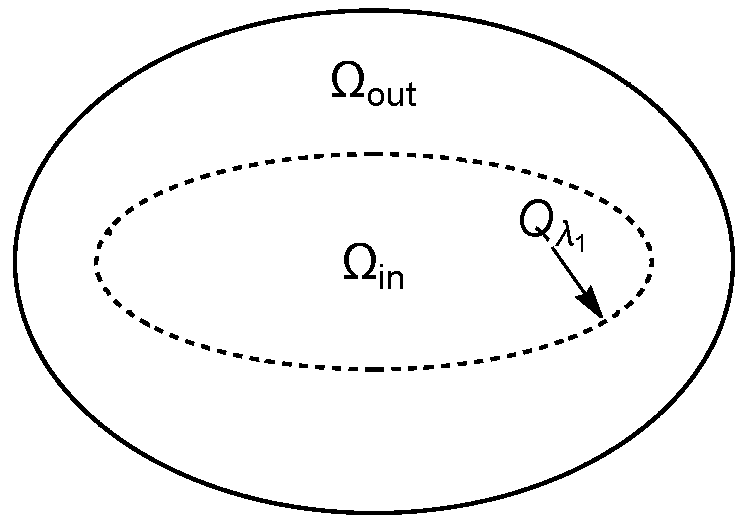
\includegraphics[scale=0.3]{images/ch4/section2/domain_problemA.pdf}
    \caption{Область $\Omega$ для задачи А.}
    \label{fig:intro_problemA}
\end{figure}

Для этой системы отрезки произвольной траектории, лежащие в области $\Omega_{in}$, касаются квадрики с параметром $\alpha_{in} \in (\lambda_1, a^2)$, а ее отрезки, лежащие в $\Omega_{out}$ -- вообще говоря, другой квадрики с параметром $\alpha_{out} \in (0, a^2)$. При этом параметры связаны соотношением $(\alpha_{out} - \lambda_1) n_{out}^2 = (\alpha_{in} - \lambda_1) n_{in}^2$.
Это тождество позволяет построить отображение $\alpha: \Xi \mapsto  L \in \mathbb{R}^2$ -- на прямую в плоскости с декартовыми координатами $(\alpha_{in}, \alpha_{out})$. 
А именно, для фиксированных $\lambda_1, n_{in}, n_{out}$ точка $\alpha(\Xi)$ лежит на прямой $L$, которая в декартовых координатах $(\alpha_{in}, \alpha_{out})$ задается уравнением
\begin{equation}
\alpha_{out} = \alpha_{in} \left(\frac{n_{in}}{n_{out}}\right)^2 + \lambda_1 \frac{n_{out}^2 - n_{in}^2}{n_{out}^2}.
\label{eq:L_line}
\end{equation}
Отметим, что прямая $L$ проходит через точку $(\alpha_{in}, \alpha_{out}) = (\lambda_1, \lambda_1)$.
Мы введем структурную диаграмму критических значений первого интеграла $\Xi$. 
\begin{figure}[!htb]
\centering
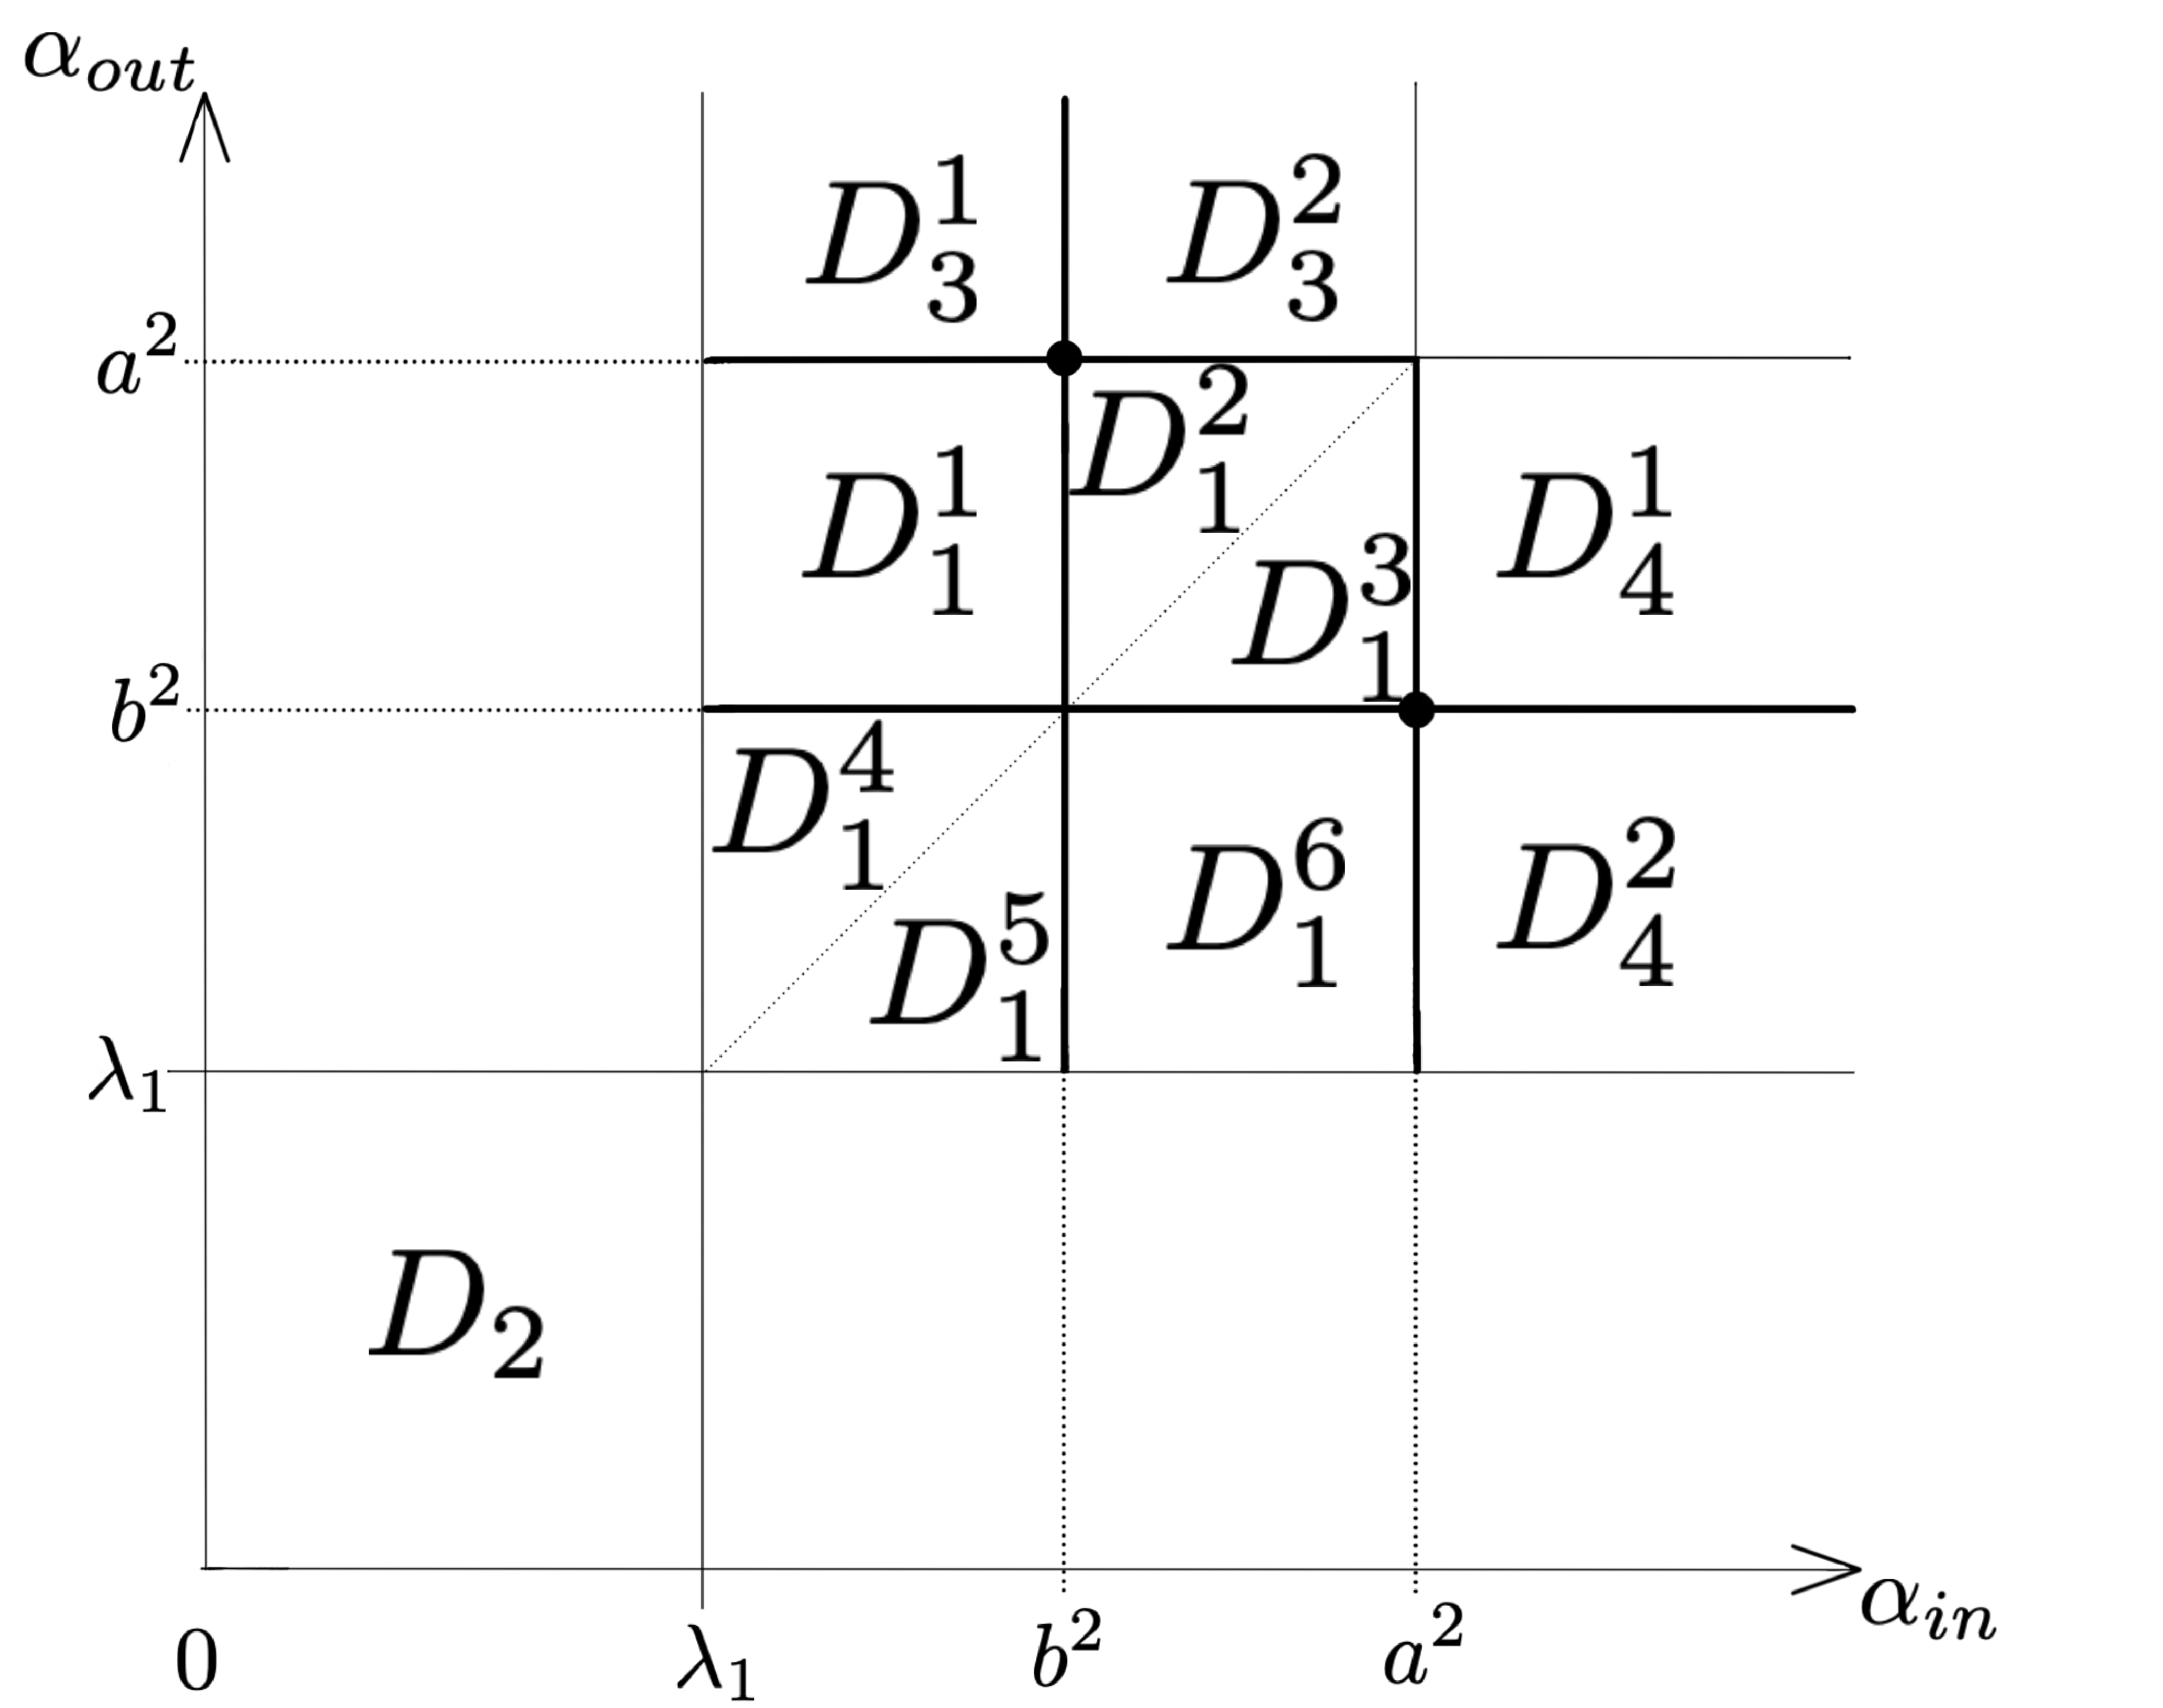
\includegraphics[scale=0.1]{images/ch4/section2/problemA_subdivisions.pdf}
    \caption{Подразбиение областей $D_1, \ldots, D_4$.}
    \label{fig:intro_problemA_subdivisions}
\end{figure}

Анализ слоения на поверхности уровня интеграла $\Xi$ проходит по следующей схеме. Сначала фиксируются параметры $\lambda_1, n_{in}, n_{out}$. Они определяют прямую $L$, при этом значение интерграла $\Xi$ однозначно определяет точку на этой прямой. Прямая $L$ пересекает некоторые области, изображенные на рис. \ref{fig:intro_problemA_subdivisions}. Разбиение на рисунке связано с различными типами траекторий (например, возможны траектории, для которых не определен $\alpha_{in}$ или $\alpha_{out}$).
Структура слоения определяется тем, как прямая $L$ пересекает изображенные области.
При этом нерегулярные значения интеграла $\Xi$ соответствуют точкам пересечения прямой $L$ с координатными линиями $\alpha_{in}, \alpha_{out} = b^2, a^2$. 
В главе доказана следующая теорема:
%Для удобства занумеруем регулярные области значений интеграла $\Xi$ на рис. \ref{fig:intro_causticTypesDiagram}.
%В ходе их описания мы узнаем как выглядят соответствующие области $\Omega$. Потом, когда будем описывать бифуркации, 
\begin{theorem} 
Областям $D_i^j$ в плоскости $(\alpha_{in}, \alpha_{out})$ соответствуют следующие поверхности $\Xi = \const$
\medskip
\begin{center}
\begin{tabular}{|c|c|c|}
\hline 
$D_1^1$  	& 	$\alpha_{in} \in (\lambda_1, b^2), \ \alpha_{out} \in (b^2, a^2)$			& сфера с 5 ручками; \\ \hline 
$D_1^2$  	& 	$\alpha_{in} \in (b^2, a^2), \ \alpha_{out} \in (\alpha_{in}, a^2)$				& сфера с 5 ручками; \\ \hline 
$D_1^3$  	& 	$\alpha_{in} \in (b^2, a^2), \ \alpha_{out} \in (b^2, \alpha_{in})$				& сфера с 5 ручками; \\ \hline 
$D_1^4$ 	& 	$\alpha_{in} \in (\lambda_1, b^2), \ \alpha_{out} \in (\alpha_{in}, b^2)$	& 2 дизъюнктных тора; \\ \hline 
$D_1^5$  	& 	$\alpha_{in} \in (\lambda_1, b^2), \ \alpha_{out} \in (\lambda_1, \alpha_{in})$	& 2 дизъюнктных тора; \\ \hline 
$D_1^6$  	& 	$\alpha_{in} \in (b^2, a^2), \ \alpha_{out} \in (\lambda_1, b^2)$			& сфера с 5 ручками; \\ \hline 
\hline
$D_2$  	& 	$(\alpha_{out} \in (0, \lambda_1), \ \alpha_{in} < \lambda_1)$ или & \\
		&  $(\alpha_{in} \in (0, \lambda_1), \ \alpha_{out} < \lambda_1)$				& 2 дизъюнктных тора; \\ \hline
 \hline
$D_3^1$  	& 	$\alpha_{in} \in (\lambda_1, b^2), \ \alpha_{out} > a^2$				& 2 дизъюнктных тора; \\ \hline 
$D_3^2$  	& 	$\alpha_{in} \in (b^2, a^2), \ \alpha_{out} > a^2 $					& 1 тор; \\ \hline 
\hline 
$D_4^1$  	& 	$\alpha_{in} > a^2, \ \alpha_{out} \in (b^2, a^2)$						& 2 дизъюнктных тора; \\ \hline 
$D_4^2$  	& 	$\alpha_{in} > a^2, \alpha_{out} \in (\lambda_1, b^2)$				& 2 дизъюнктных тора; \\ \hline 
\end{tabular}
\end{center}
\label{st:intron1_n2_surfaces}
\end{theorem} 
В завершение приведены особые поверхности, соответствующие пересечению прямой $L$ и выделенных на рис. \ref{fig:intro_problemA_subdivisions} сегментов координатных линий $\alpha_{in}, \alpha_{out} = b^2, a^2$. Приведенные 13 бифуркаций включают в себя <<двойные перестройки>>, соответствующие пересечению прямой $L$ с точками  $(b^2, a^2)$ и $(a^2, b^2)$. Для нетривиальных особых поверхностей приведены иллюстрации.



\underline{\textbf{Пятая глава}} посвящена рассмотрению задачи Б: описать слоения изоэнергитического многообразия на поверхности уровня первого интеграла $\Xi$ для подчиняющейся закону $(\ast)$ бильярдной системы в области $\Omega = \Omega_1 \cup \Omega_2$ (см. рис. \ref{fig:intro_domain}). Показатели преломлений $n_1$ для $\Omega_1$ и $n_2$ для $\Omega_2$ предполагаем фиксированными.
\begin{figure}[!htb]
\centering
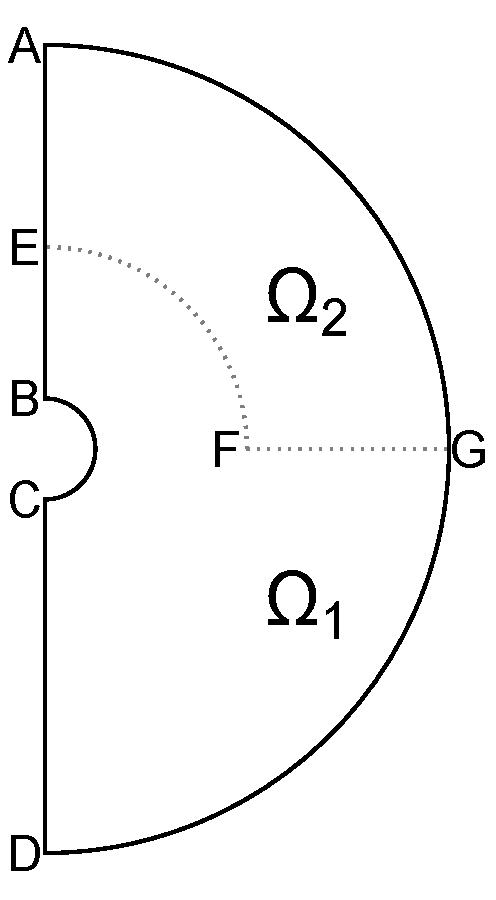
\includegraphics[scale=0.3]{images/ch4/section3_circular/domain.pdf}
    \caption{Область $\Omega$ представляет собой объединение 2 областей.}
    \label{fig:intro_domain}
\end{figure}
Для этой системы в качестве постоянной движения, сохраняющейся в областях $\Omega_1$ и $\Omega_2$ до пересечения дуг $EF$ или $FG$ рассматривается величина $\rho^2 =  \frac{(x v_y - y v_x)^2}{v_x^2 + v_y^2}$. При этом на двух границах раздела сред $EF$ и $FG$ параметр каустики $\rho^2$ преобразуется по-разному:
\begin{statement}
Имеют место следующие соотношения для параметров $\rho_1, \rho_2$ в точке преломления:
\begin{align}
(\rho_1^2 - r_1^2)n_1^2 = (\rho_2^2 - r_1^2)n_2^2 \qquad & 
			\text{ при } (x,y) \in EF, 
			\label{eq:st1_eq1}
			\\
\rho_1^2 n_1^2 = \rho_2^2 n_2^2 \qquad  & \text{ при } (x,y) \in FG.
			\label{eq:st1_eq2}
\end{align}
\label{st:across_EF}
\end{statement}

Разобьем бильярдную траекторию в точках пересечения дуги $EF$ на фрагменты $T_k, k \geq 1$. 
Каждый фрагмент бильярдной траектории $T_k$ образует ломаную кривую в $\Omega \setminus EF$, где $EF  \subset \partial \Omega_1 \cap \partial \Omega_2$.
Введем на $\Omega \setminus EF$ функцию $\Xi(x, y, v_x, v_y)$ по формуле
\begin{equation}
\Xi(x, y, v_x, v_y) = \left[
\begin{array}{ll}
    \rho^2(x,y,v_x,v_y) n_1^2, &  \text{ если } (x,y) \in \Omega_1 \\
    \rho^2(x,y,v_x,v_y) n_2^2, & \text{ если } (x,y) \in \Omega_2.
\end{array}
\right.
\label{eq:XiDefinition}
\end{equation}
Эта функция постоянна в каждой точке фрагмента бильярдной траектории $T_k$, но на разных фрагментах значения могут различаться. 

Направления роста и убывания интеграла $\Xi$ можно проиллюстрировать на примере рис. \ref{fig:n1gtn2_Xi_growth} и \ref{fig:n1ltn2_Xi_growth}.
\begin{figure}[!htb]
\minipage{0.5\textwidth}
\centering
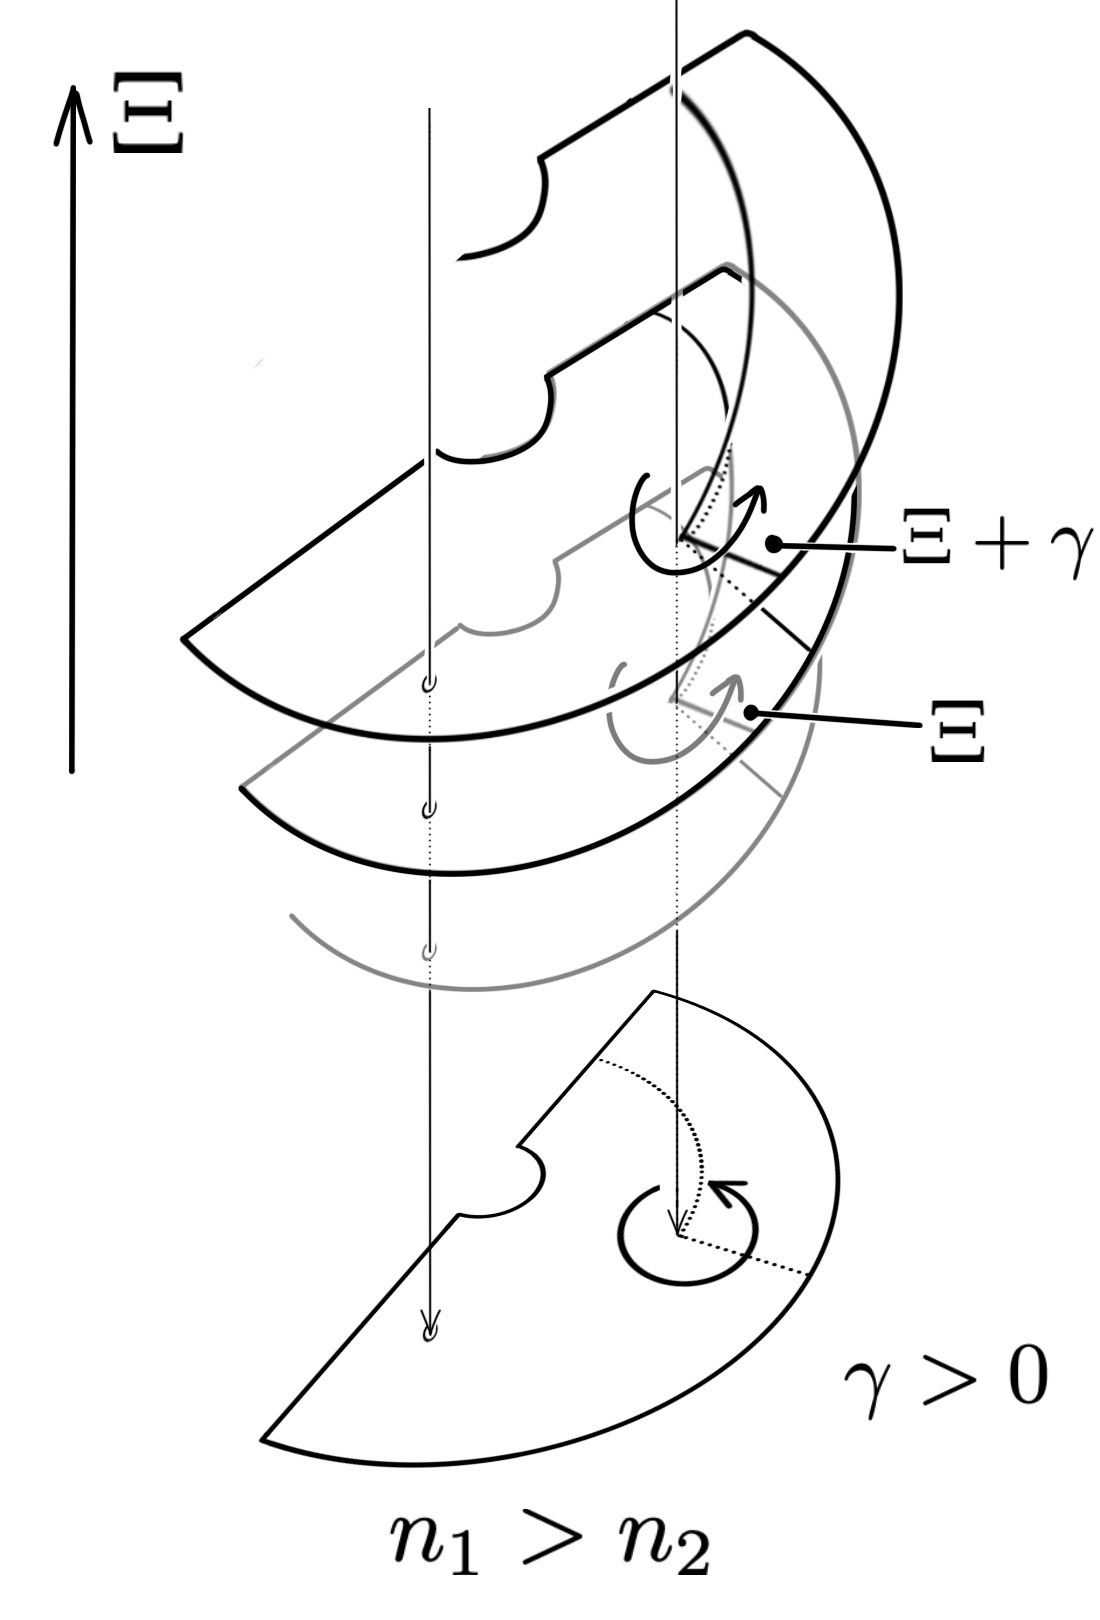
\includegraphics[width=5cm]{images/ch4/section3_circular/n1gtn2.png}
    \caption{Направление роста $\Xi$ при $n_1 > n_2$.}
    \label{fig:n1gtn2_Xi_growth}
\endminipage\hfill
\minipage{0.5\textwidth}
\centering
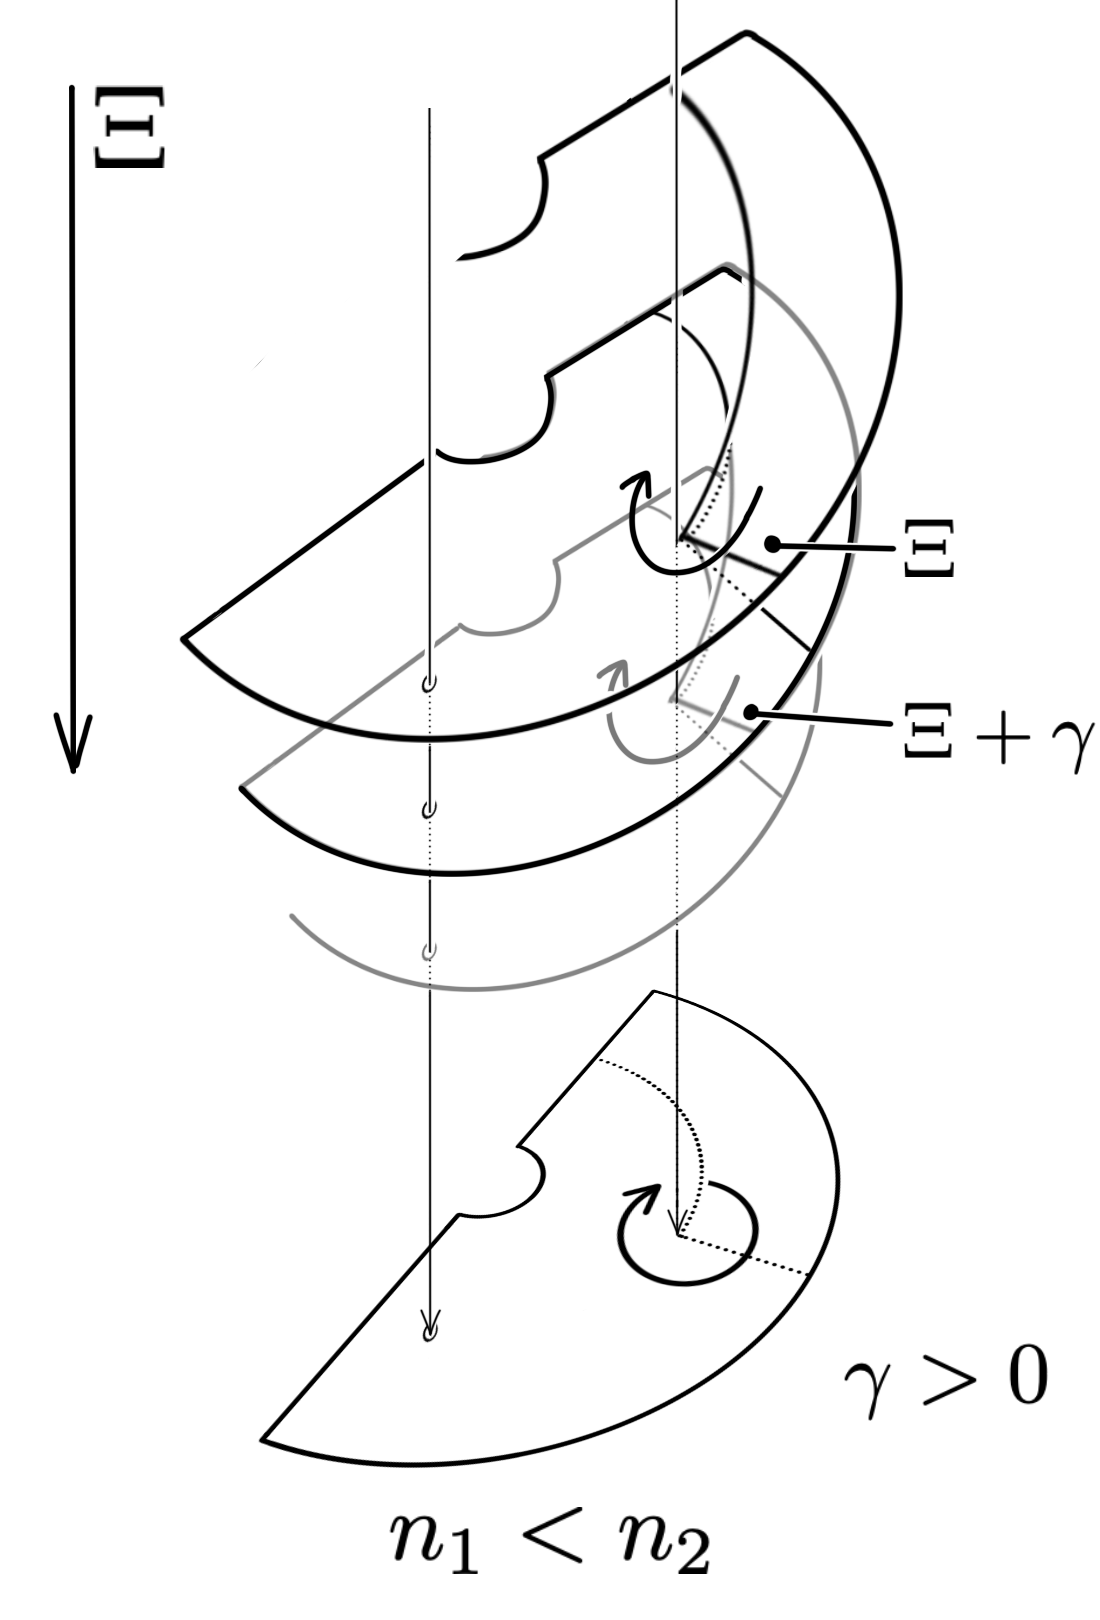
\includegraphics[width=5cm]{images/ch4/section3_circular/n1ltn2.png}
    \caption{Направление роста $\Xi$ при $n_1 < n_2$.}
    \label{fig:n1ltn2_Xi_growth}
\endminipage\hfill
\end{figure}

Рассмотрим значения интеграла $\Xi$ для двух последовательных фрагментов $T_k, T_{k+1}$. Выясним, как они связаны, или, что то же самое, как меняется интеграл $\Xi$ при преломлении на дуге $EF$. 

\begin{statement}
Значения $\Xi_k$ и $\Xi_{k+1}$  интеграла $\Xi$, соответствующие фрагментам траектории $T_k$ и $T_{k+1}$, различаются на величину $r_1^2(n_1^2-n_2^2)$.
\end{statement}
Значению интеграла $\Xi$ поставим в соответствие точку плоскости $\mathbb{R}^2$ по формуле 
\begin{equation}
\Xi \mapsto P(\Xi) = (\rho_1^2, \rho_2^2) = \left( \frac{\Xi}{n_1^2}, \frac{\Xi}{n_2^2} \right).
% = \left( \left. \rho^2 \right|_{\Omega_1} ,  \left. \rho^2 \right|_{\Omega_2}  \right).
\label{eq:XiMap}
\end{equation}
Тогда для фиксированных параметров $n_1, n_2$ отображением $P$ значения величины $\Xi$ отображаются на прямую $L \subset \mathbb{R}^2$. 
Параметризуем прямую $L: \xi \mapsto P(\xi) = (\xi \cos \theta, \xi \sin \theta)$. На ней можно выделить точку $L_1$, которая разделяет прямую на две части относительно параметра $\xi$ на прямой $L$ на две части: $\{ \xi < L_1\}$ и $\{ \xi > L_1\}$. Объединяя эти части по всевозможным прямым $L$, получим области в $\mathbb{R}^2$, изображенные на рис. \ref{fig:pt10:_lineDomains_simple}.
\begin{figure}[!htb]
\centering
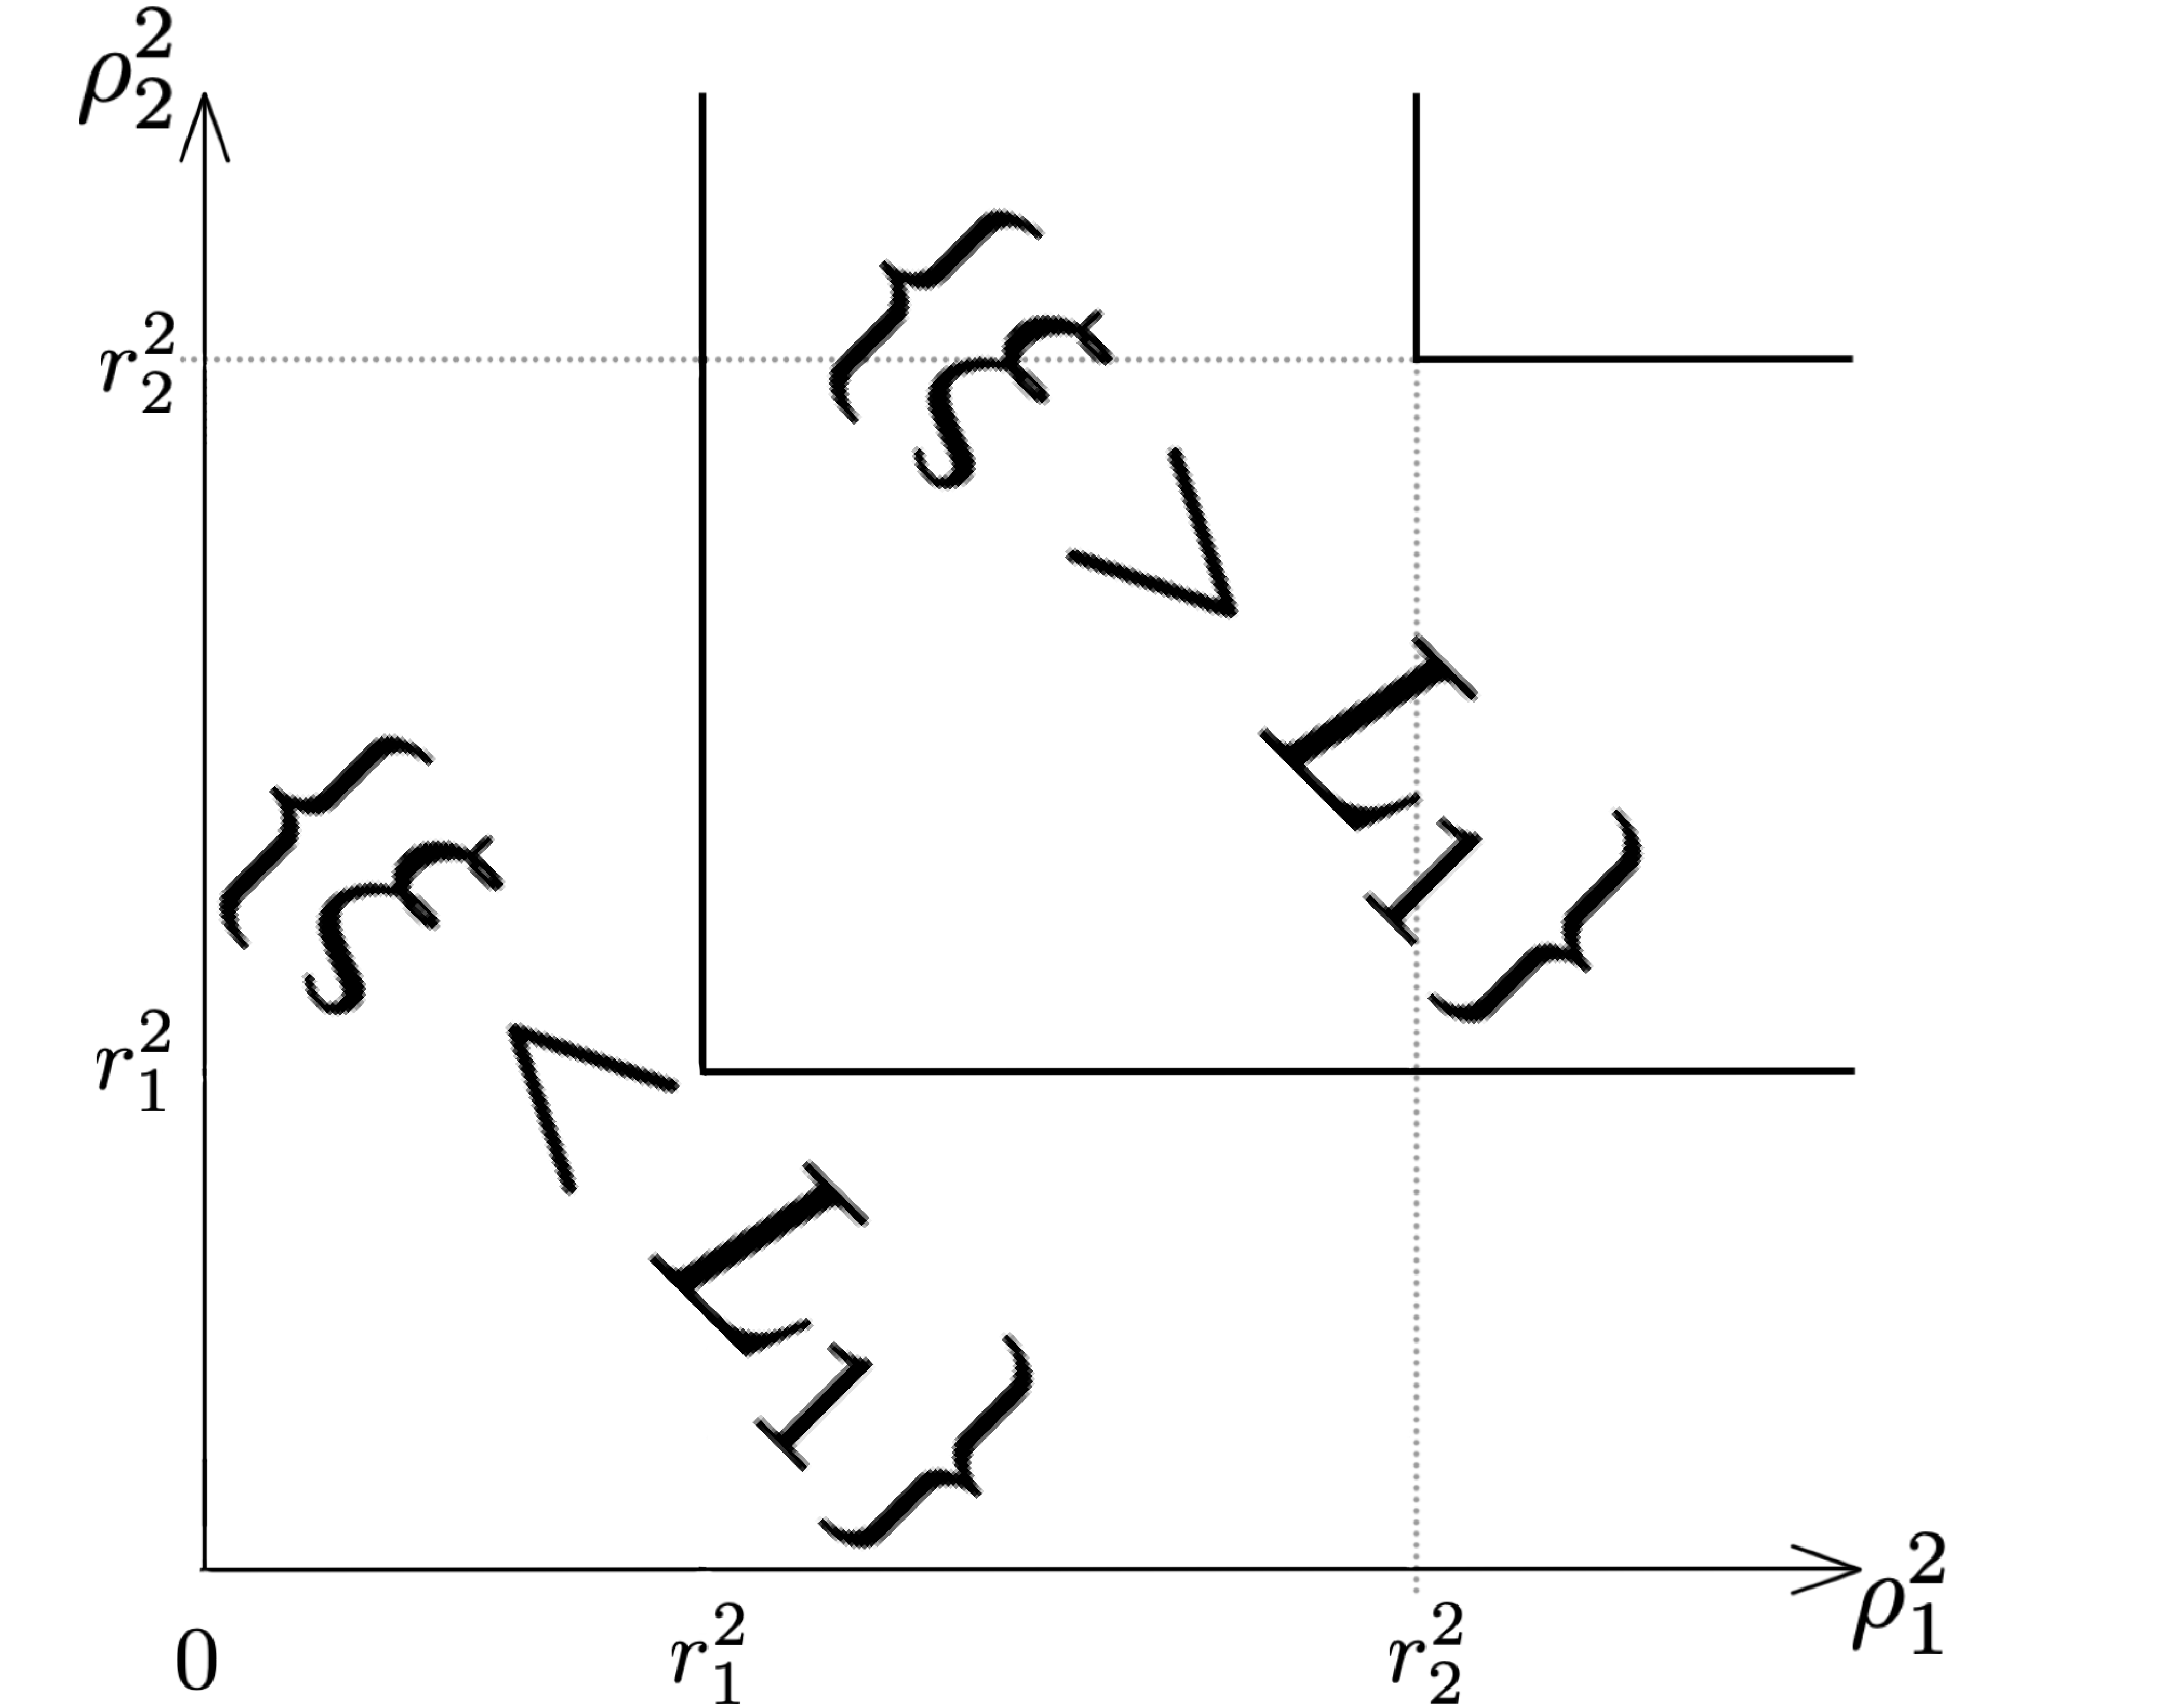
\includegraphics[scale=0.07]{images/ch4/section3_circular/line_domains_simple.pdf}
    \caption{Области $\left\{\xi< L_1\right\}$ и $\left\{\xi > L_1\right\}$.}
    \label{fig:pt10:_lineDomains_simple}
\end{figure}
При этом показано, что эти множества являются непересекающимися в смысле бильярдных траекторий: если траектория пересекает $EF$ хотя бы однажды, тогда точки, соответствующие фрагментам $T_k$ такой траектории, находятся только на части прямой $L$, попадающей внутрь области $\{ \xi < L_1\}$, изображенной на рис. \ref{fig:pt10:_lineDomains_simple}.
Эти области рассматриваются отдельно в соответствующих разделах главы.


Для области $\{\xi < L_1\}$, соответствующей <<ветвящемуся интегралу>>, получена бифуркационная диаграмма (см. рис. \ref{fig:pt10:_B1_lattice_straight}), на которой фрагмент $L \cap \{\xi < L_1\}$ выглядит как горизонтальная прямая. 
\begin{figure}[!htb]
\centering
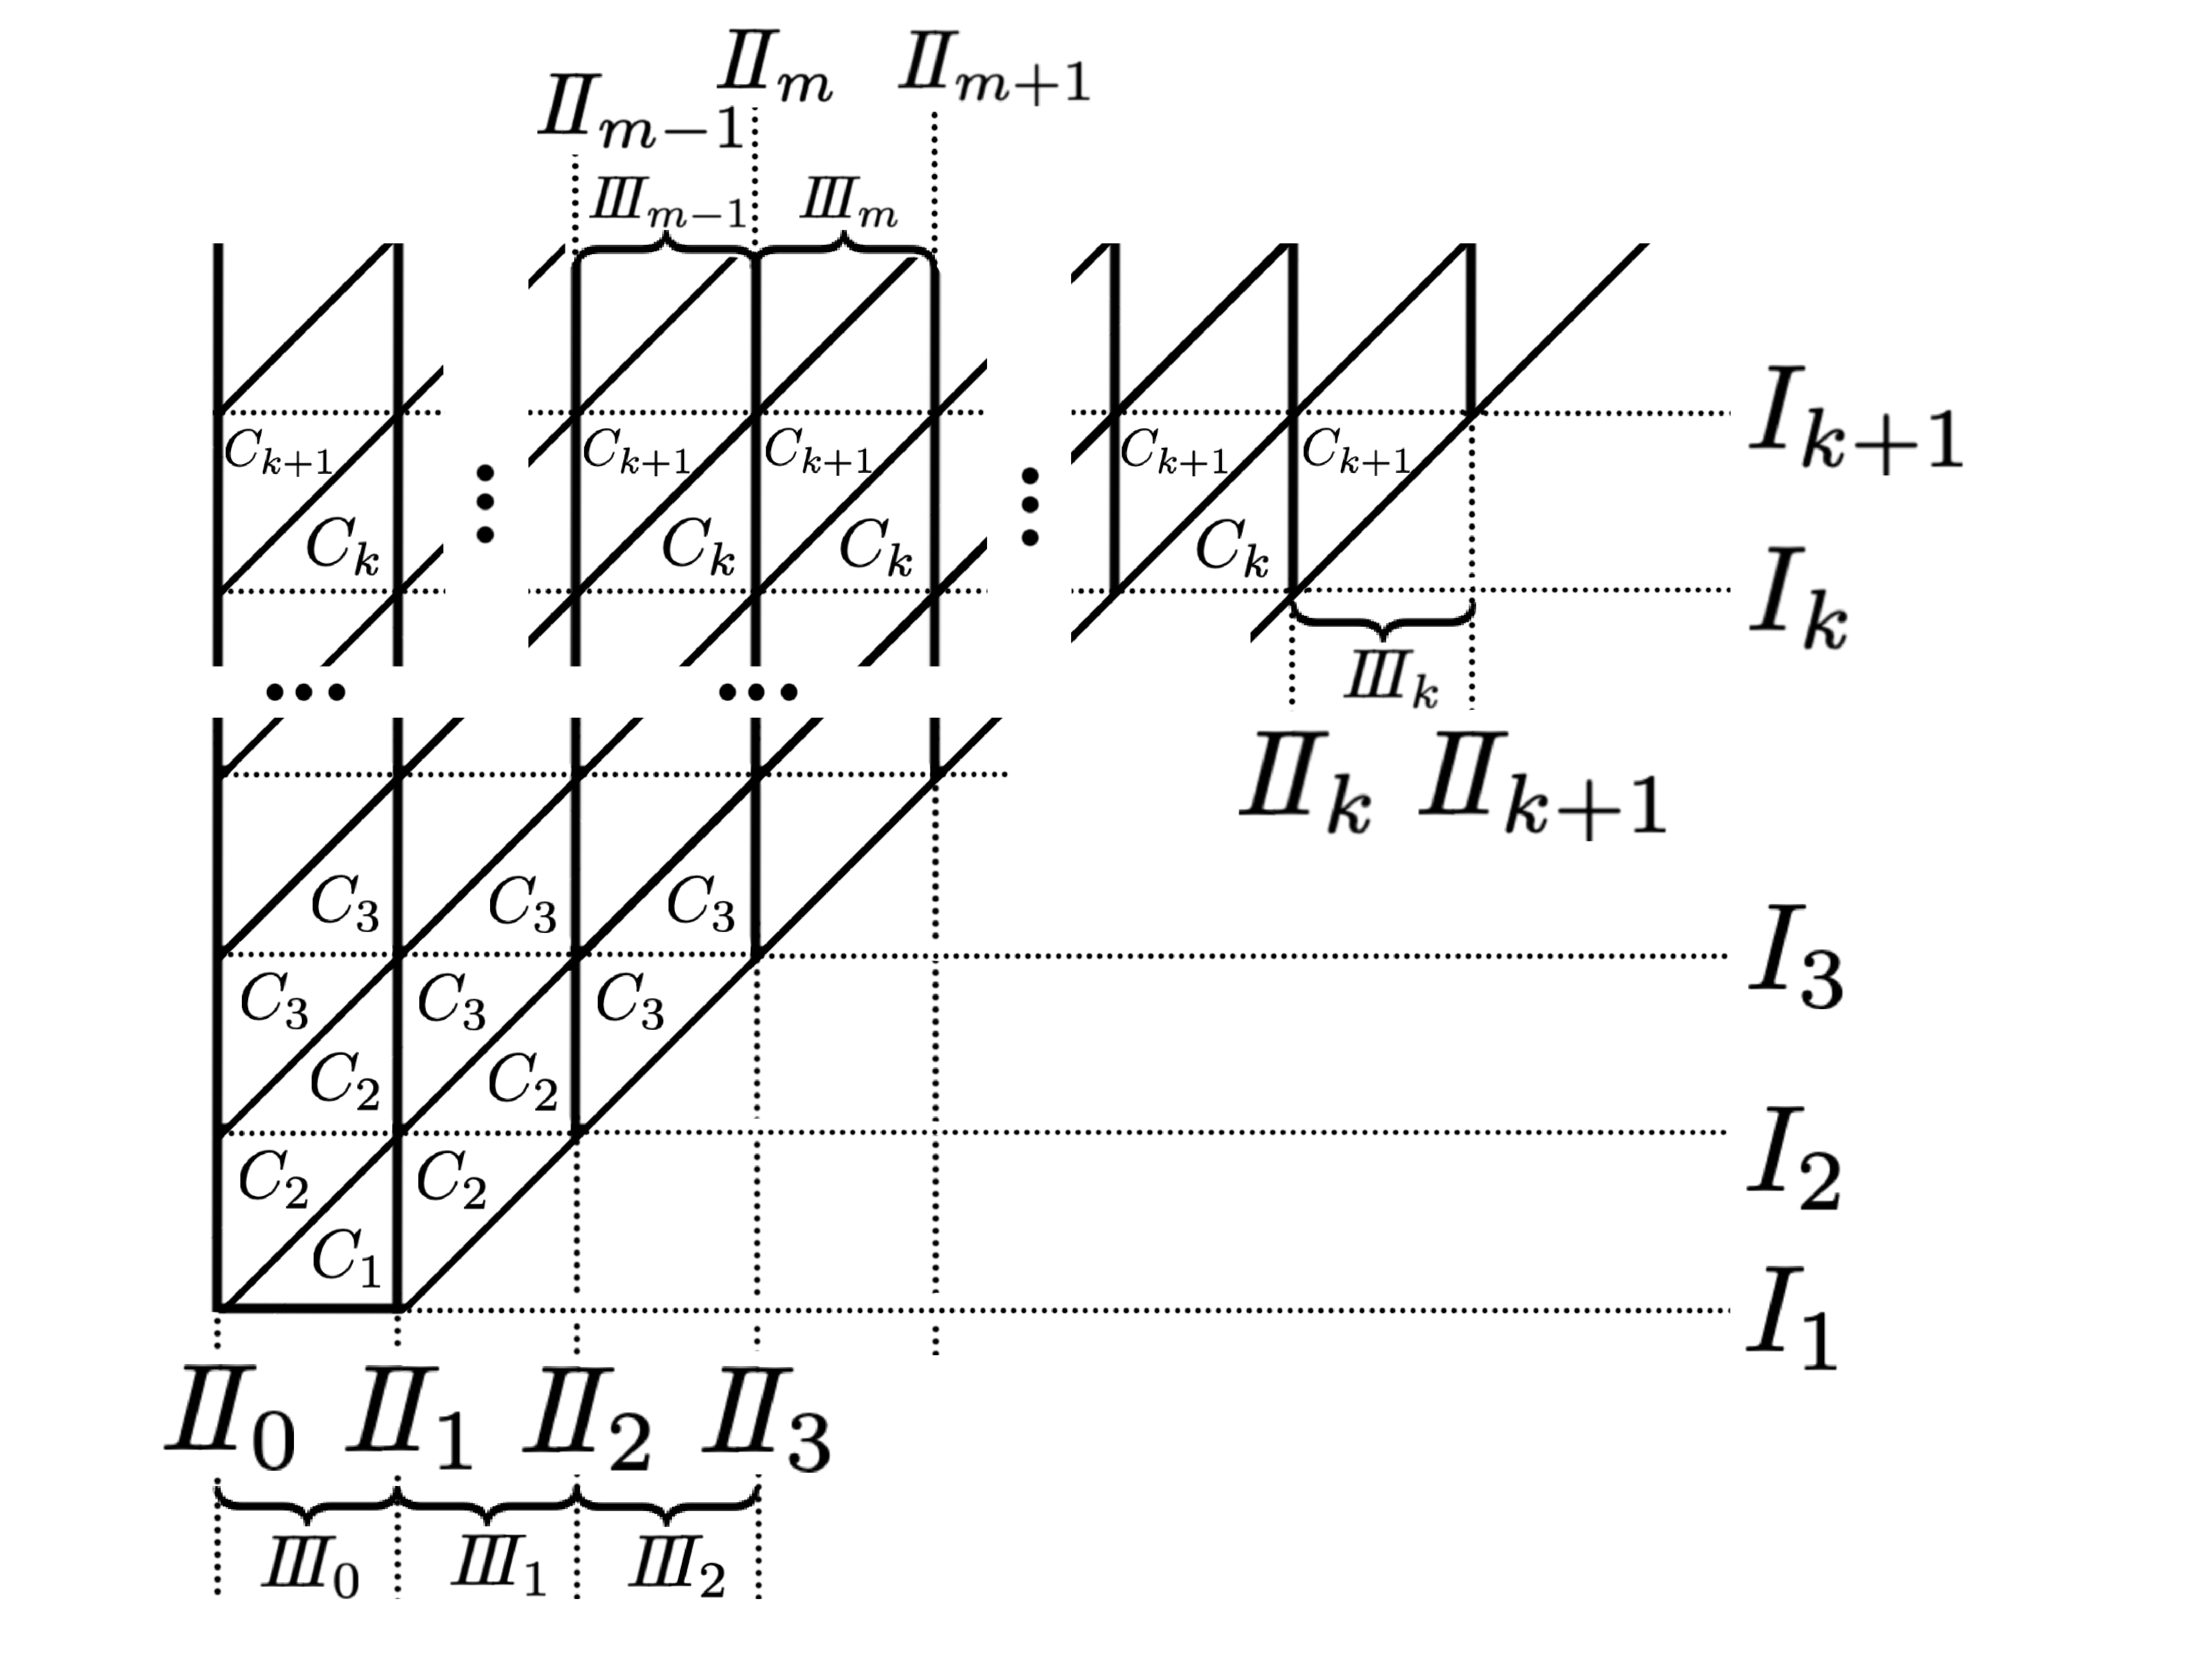
\includegraphics[width=10cm]{images/ch4/section3_circular/B1_lattice_straight.pdf}
    \caption{}
    \label{fig:pt10:_B1_lattice_straight}
\end{figure}
При этом для любой фиксированной тройки параметров $(r_1, n_1, n_2)$ точки $P(\Xi_m)$ и $P(\Xi_{m+1})$, соответствующие двум последовательным фрагментам бильярдной траектории $T_m$ и $T_{m+1}$, соединяются вектором $(1, 0)$. 
Структура слоения определяется тем, как прямая $L \cap \{\xi < L_1\}$ пересекает области, обозначенные $C_k, k \geq 1$ на рис. \ref{fig:pt10:_B1_lattice_straight}. 
При этом в склейке регулярных поверхностей участвуют все $C_m$ одного и того же индекса $m$, лежащие на одной горизонтали. Нерегулярным поверхностям соответствуют точки пересечения прямой $L \cap \{\xi < L_1\}$ с прямыми одного из трех семейств, отмеченных римскими цифрами.

Приводится классификация заметаемых областей для фрагментов бильярдных траекторий $T_m$ в зависимости от расположения соответствующей точки $P(\Xi_m)$ на диаграмме (см. рис. \ref{fig:pt10:_B1Prime_lattice}).
\begin{figure}[!htb]
\centering
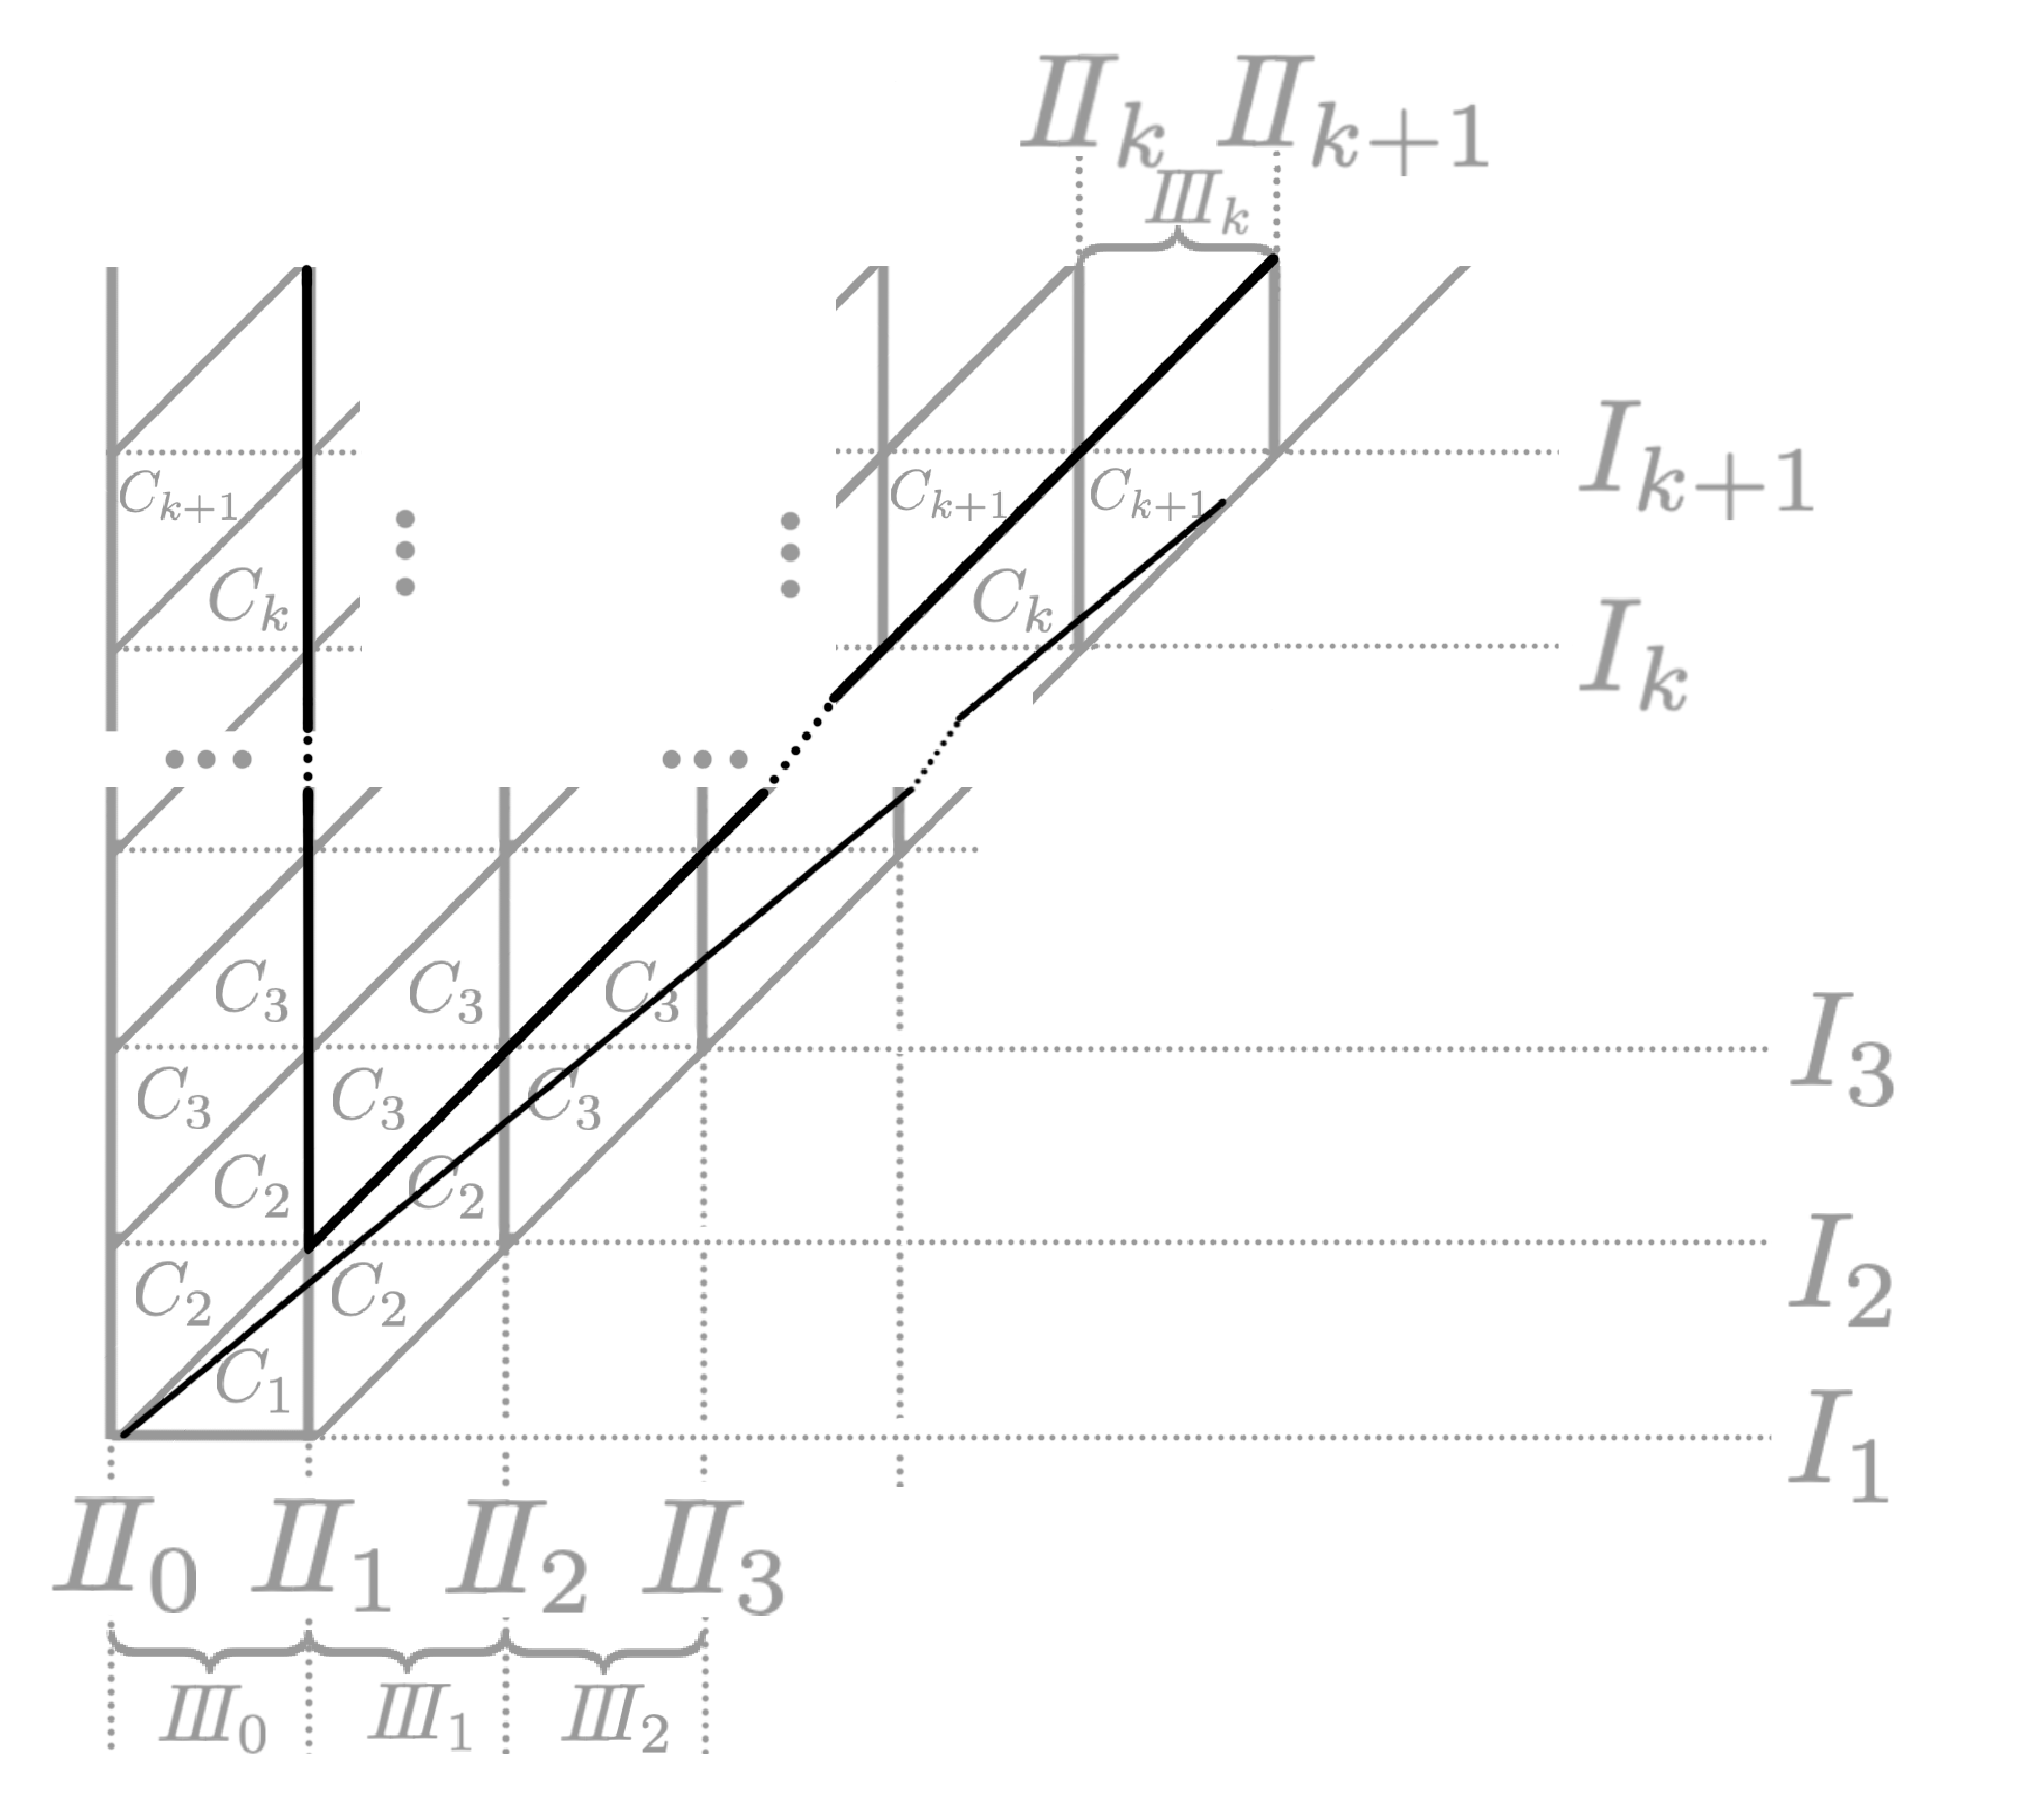
\includegraphics[width=7cm]{images/ch4/section3_circular/B1Prime_lattice.pdf}
    \caption{Прямая, соответствующая прямой $\rho_1^2 = r_2^2$.}
    \label{fig:pt10:_B1Prime_lattice}
\end{figure}
Для неособых поверхностей доказаны следующие теоремы:
\textit{При $n_1^2<n_2^2$}
\begin{theorem}
В области $\left\{\xi < L_1\right\}$ поверхности $S_\Xi$ являются сферами с $2m$ ручками, если $P(\Xi) \in C_m$ и сферами с $2m-1$ ручками, если $P(\Xi) \in C_m'$ и $m \leq \left\lfloor \frac{r_2^2}{r_2^2-r_1^2} \right\rfloor$. 
\label{th:pt10:th1}
\end{theorem}
\textit{При $n_1^2 > n_2^2$}
\begin{theorem}
В области $\left\{\xi < L_1\right\}$ поверхности $S_\Xi$ являются сферами с $2m+1$ ручками, если $P(\Xi) \in C_m$ и сферами с $2m$ ручками, если $P(\Xi) \in C_m'$ и $m \leq \left\lfloor \frac{r_2^2}{r_2^2-r_1^2} \right\rfloor$. 
\label{th:pt10:th2}
\end{theorem}

Случай $\{\xi > L_1\}$ существенно проще предыдущего, поскольку в этом случае дополнительный интеграл $\Xi$ однозначен: бильярдные траектории лежат на поверхностях уровня дополнительного интеграла $\Xi=\const$.
Структура слоения определяется тем, как прямая $L \cap  \{\xi > L_1\}$ пересекает четыре области, изображенные на рис. \ref{fig:pt10:_xiL1_subdivision}.
\begin{figure}[!htb]
\centering
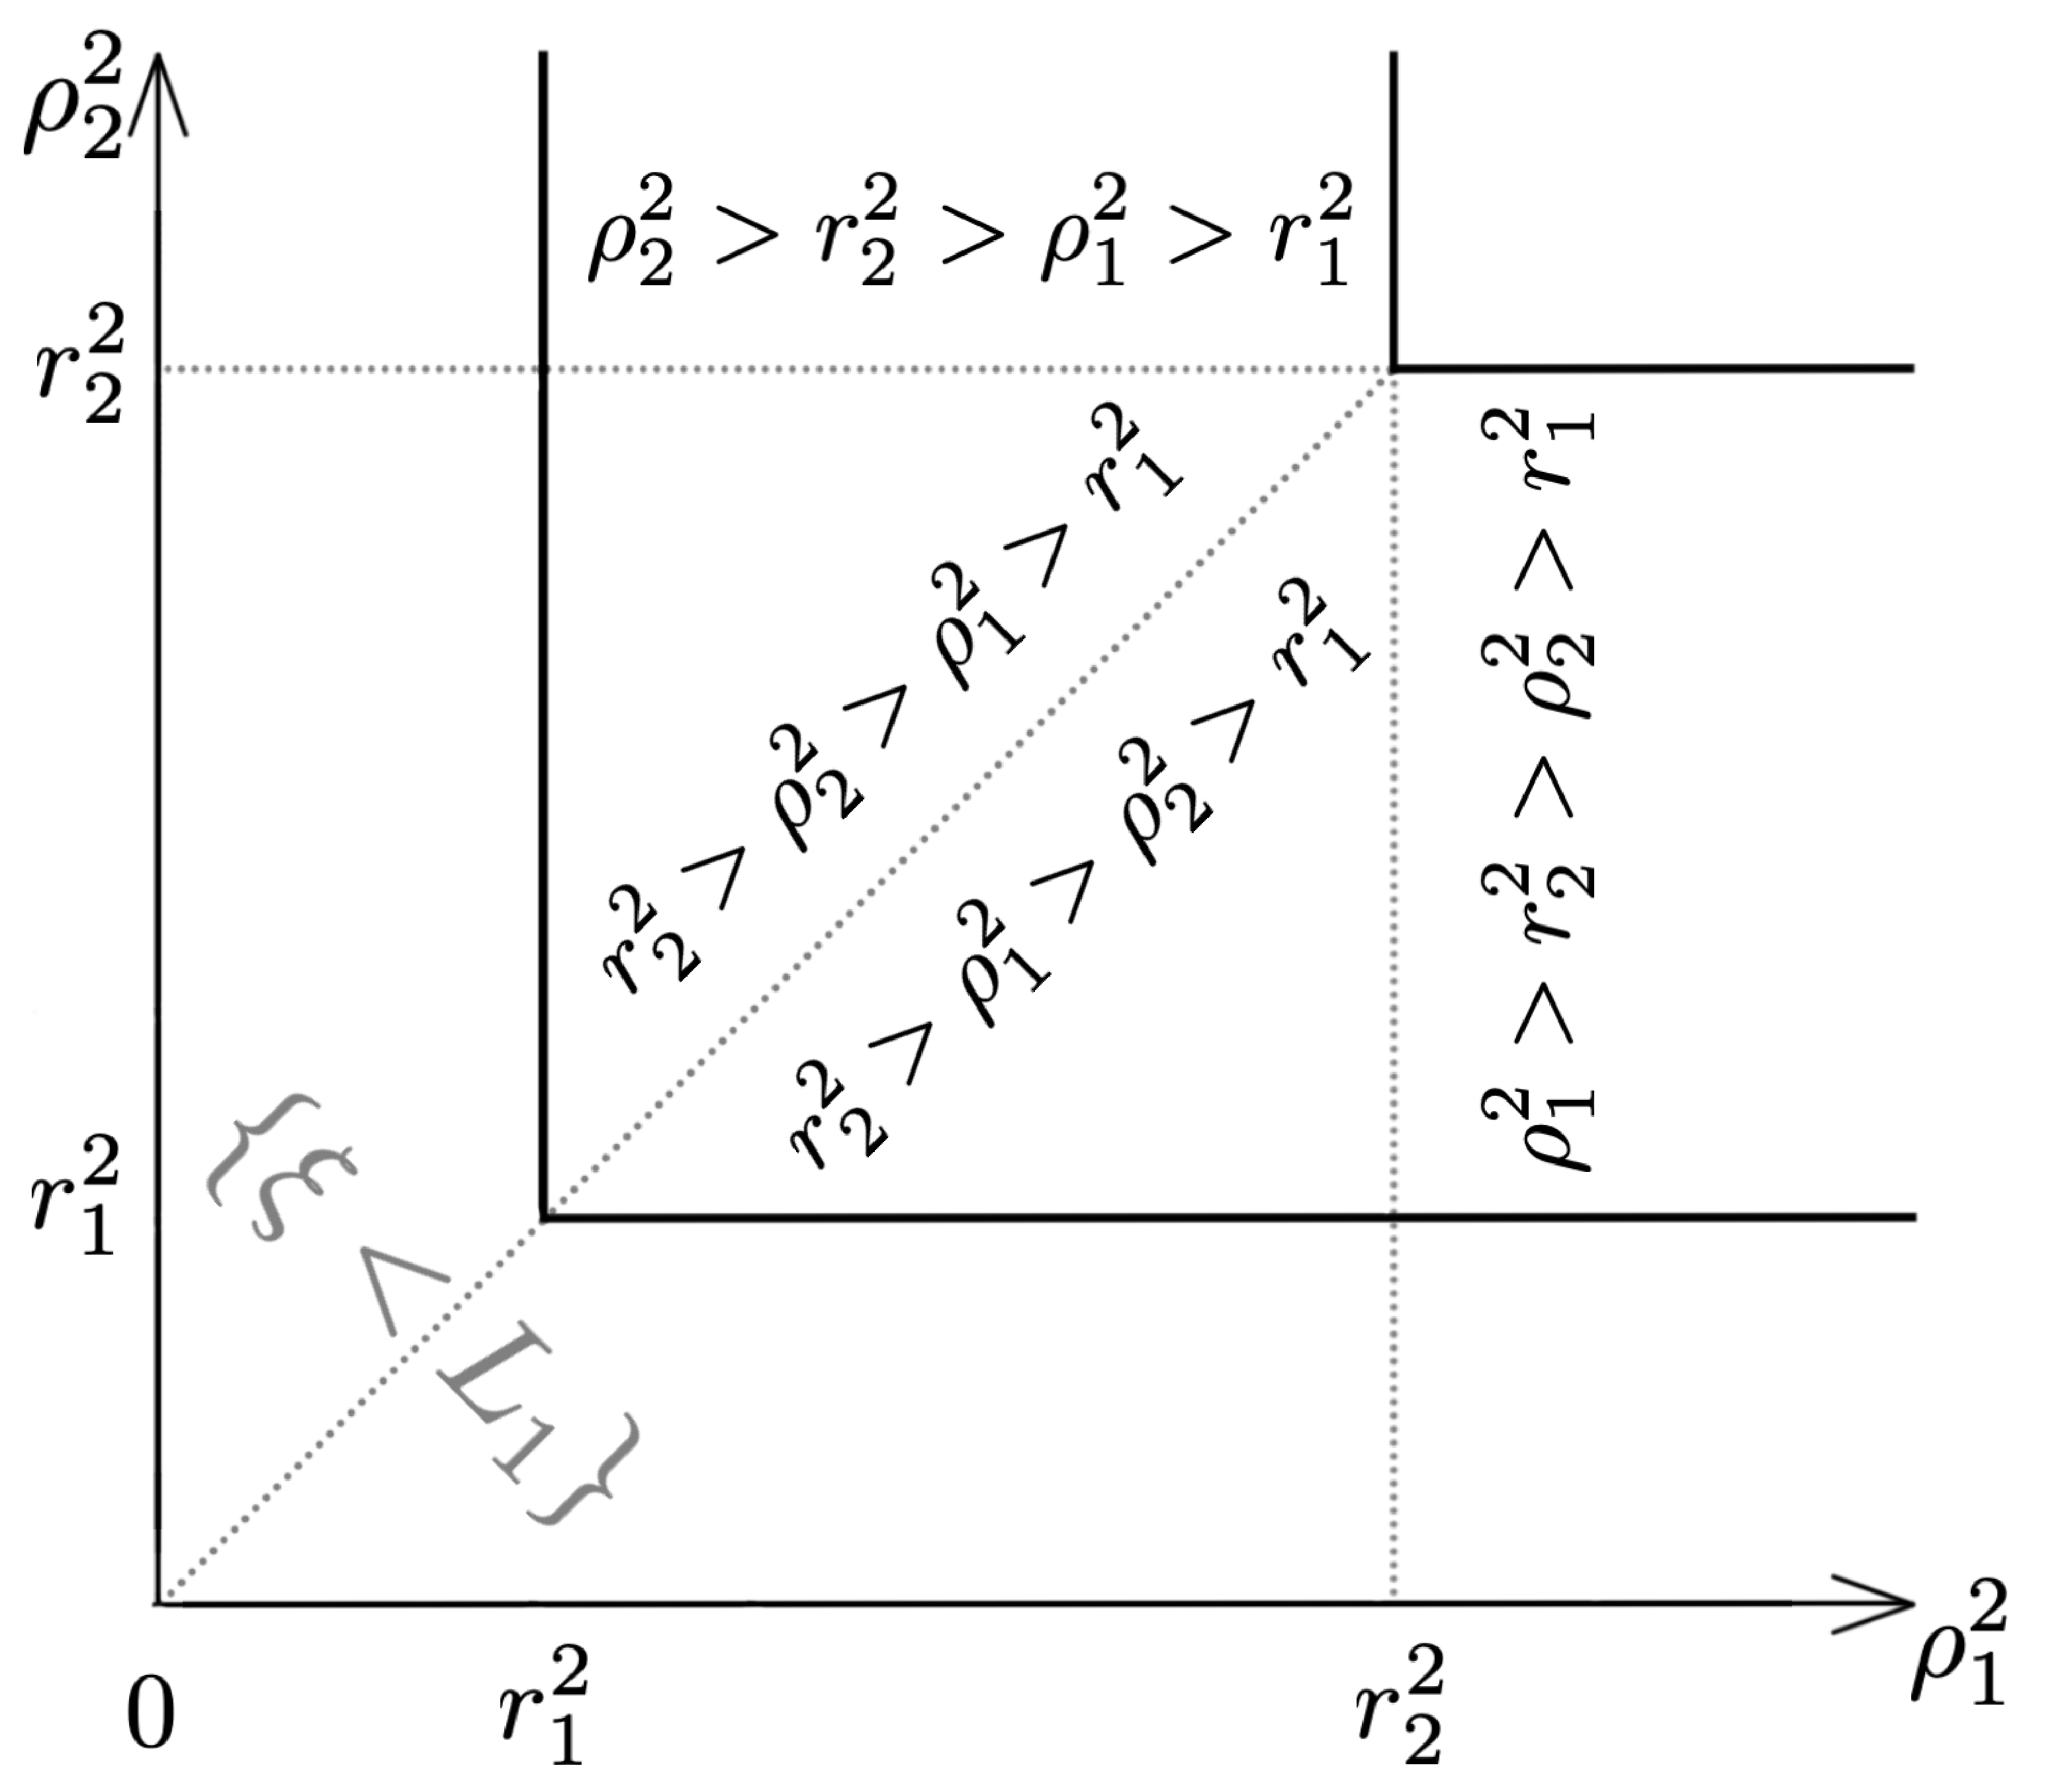
\includegraphics[width=6cm]{images/ch4/section3_circular/sect3_xiL1_subdivision.pdf}
    \caption{Разбиение области $\left\{\xi > L_1\right\}$.}
    \label{fig:pt10:_xiL1_subdivision}
\end{figure}
Доказано следующее:
\begin{theorem}
Поверхность уровня $\Xi = \const$ является сферой с двумя ручками для случаев
\begin{itemize}[beginpenalty=10000]
\item $r_2^2 > \rho_1^2 > \rho_2^2 > r_1^2$
\item $r_2^2 > \rho_2^2 > \rho_1^2 > r_1^2$
\end{itemize}
И тором для случаев 
\begin{itemize}[beginpenalty=10000]
\item $\rho_2^2 > r_2^2 > \rho_1^2 > r_1^2$
\item $\rho_1^2 > r_2^2 > \rho_2^2 > r_1^2$
\end{itemize}
\end{theorem}

В завершение главы приводятся описания особых поверхностей для случаев $\{\xi < L_1\}$ и $\{\xi > L_1\}$ с иллюстрациями для ключевых перестроек.

\FloatBarrier
\pdfbookmark{Заключение}{conclusion}                                  % Закладка pdf
В \underline{\textbf{заключении}} перечислены основные результаты диссертации, а также предложены
возможные направления дальнейших исследований в рамках тематики работы.

{\gratitude}
Автор выражает глубокую благодарность своему научному руководителю Ф.Ю.Попеленскому за постановку задачи, постоянную поддержку и внимание к работе на всех этапах её подготовки. 
Автор благодарит коллектив кафедры дифференциальной геометрии и приложений механико-математического факультета МГУ за вдохновляющую, доброжелательную атмосферу и поддержку.

%{\gratitude}
%\pdfbookmark{Литература}{bibliography}                                % Закладка pdf
%При использовании пакета \verb!biblatex! список публикаций автора по теме
%диссертации формируется в разделе <<\publications>>\ файла
%\verb!common/characteristic.tex!  при помощи команды \verb!\nocite!
%\insertbiblioauthor

\ifdefmacro{\microtypesetup}{\microtypesetup{protrusion=false}}{} % не рекомендуется применять пакет микротипографики к автоматически генерируемому списку литературы
\urlstyle{rm}                               % ссылки URL обычным шрифтом
\ifnumequal{\value{bibliosel}}{0}{% Встроенная реализация с загрузкой файла через движок bibtex8
    \renewcommand{\bibname}{\large \bibtitleauthor}
    \nocite{*}
    \insertbiblioauthor           % Подключаем Bib-базы
    %\insertbiblioexternal   % !!! bibtex не умеет работать с несколькими библиографиями !!!
}{% Реализация пакетом biblatex через движок biber
    % Цитирования.
    %  * Порядок перечисления определяет порядок в библиографии (только внутри подраздела, если `\insertbiblioauthorgrouped`).
    %  * Если не соблюдать порядок "как для \printbibliography", нумерация в `\insertbiblioauthor` будет кривой.
    %  * Если цитировать каждый источник отдельной командой --- найти некоторые ошибки будет проще.
    %
    %% authorvak
    \nocite{vakbib1}%
    \nocite{vakbib2}%
    \nocite{vakbib3}%
    \nocite{vakbib4}%
    \nocite{vakbib5}%
    \nocite{vakbib6}%
    \nocite{vakbib7}%
    \nocite{vakbib8}%
    \nocite{vakbib9}%
    \nocite{vakbib10}%
    \nocite{vakbib11}%
    \nocite{vakbib12}%
    %
    %% authorwos
    \nocite{wosbib1}%
    %
    %% authorscopus
    \nocite{scbib1}%
    %
    %% authorpatent
    \nocite{patbib1}%
    %
    %% authorprogram
    \nocite{progbib1}%
    %
    %% authorconf
    \nocite{confbib1}%
    \nocite{confbib2}%
    %
    %% authorother
    \nocite{bib1}%
    \nocite{bib2}%

    \ifnumgreater{\value{usefootcite}}{0}{
        \begin{refcontext}[labelprefix={}]
            \ifnum \value{bibgrouped}>0
                \insertbiblioauthorgrouped    % Вывод всех работ автора, сгруппированных по источникам
            \else
                \insertbiblioauthor      % Вывод всех работ автора
            \fi
        \end{refcontext}
    }{
        \ifnum \totvalue{citeexternal}>0
            \begin{refcontext}[labelprefix=A]
                \ifnum \value{bibgrouped}>0
                    \insertbiblioauthorgrouped    % Вывод всех работ автора, сгруппированных по источникам
                \else
                    \insertbiblioauthor      % Вывод всех работ автора
                \fi
            \end{refcontext}
        \else
            \ifnum \value{bibgrouped}>0
                \insertbiblioauthorgrouped    % Вывод всех работ автора, сгруппированных по источникам
            \else
                \insertbiblioauthor      % Вывод всех работ автора
            \fi
        \fi
        %  \insertbiblioauthorimportant  % Вывод наиболее значимых работ автора (определяется в файле characteristic во второй section)
%        \begin{refcontext}[labelprefix={}]
%            \insertbiblioexternal            % Вывод списка литературы, на которую ссылались в тексте автореферата
%        \end{refcontext}
        % Невидимый библиографический список для подсчёта количества внешних публикаций
        % Используется, чтобы убрать приставку "А" у работ автора, если в автореферате нет
        % цитирований внешних источников.
        \printbibliography[heading=nobibheading, section=0, env=countexternal, keyword=biblioexternal, resetnumbers=true]%
    }
}
\ifdefmacro{\microtypesetup}{\microtypesetup{protrusion=true}}{}
\urlstyle{tt}                               % возвращаем установки шрифта ссылок URL
